\documentclass[12pt,onecolumn]{article}
\usepackage[utf8]{inputenc} % UTF8 input encoding
\usepackage[T2A]{fontenc}   % T2A font encoding for Cyrillic script
\usepackage[russian]{babel} % Russian language support
\usepackage{listings}
\usepackage{float}
\usepackage{mathtools}
\everymath{\displaystyle}
\usepackage{listings} 
\usepackage[usenames]{color}
\usepackage{geometry}
\usepackage{verbatim}
\newcommand{\nparagraph}[1]{\paragraph{#1}\mbox{}\\}
\geometry{
  a4paper,
  top=25mm, 
  right=15mm, 
  bottom=25mm, 
  left=15mm
}

\begin{document}
\setcounter{tocdepth}{4}
\begin{center}
    Федеральное государственное автономное образовательное учреждение высшего образования "Национальный Исследовательский Университет ИТМО"\\ 
    Мегафакультет Компьютерных Технологий и Управления\\
    Факультет Программной Инженерии и Компьютерной Техники \\
    
\includegraphics[scale=0.3]{image/itmo.jpg} % нужно закинуть картинку логтипа в папку с отчетом
\end{center}
\vspace{1cm}


\begin{center}
    \textbf{Модуль №1}\\
    по дисциплине\\
    \textbf{'Системы искусственного интеллекта'}
\end{center}

\vspace{2cm}

\begin{flushright}
  Выполнил Студент  группы P32101\\
  \textbf{Лапин Алексей Александрович}\\
  Преподаватель: \\
  \textbf{Авдюшина Анна Евгеньевна}\\
\end{flushright}

\vspace{6cm}
\begin{center}
    г. Санкт-Петербург\\
    2023г.
\end{center}

\newpage
\tableofcontents
\newpage

\section{Введение:}
\subsection{Описание целей проекта и его значимости.}
\paragraph{Цели проекта:}
Целью данного проекта является разработка и применение системы, основанной на базе знаний и онтологии, для поддержки пользователей в принятии решений в контексте выбора видеоигры. Проект включает в себя следующие лабораторные работы:
\paragraph{Описание лабораторных работ:}
\subparagraph{Лабораторная 1. Создание базы знаний и выполнение запросов в Prolog}
Эта лабораторная работа направлена на развитие навыков работы с фактами, предикатами и правилами в логическом программировании с использованием языка Prolog. Важными задачами являются создание базы знаний и выполнение разнообразных запросов к этой базе.
\subparagraph{Лабораторная 2. Создание онтологии в Protege}
Цель этой лабораторной работы - преобразовать базу знаний, созданную в лабораторной работе 1, в онтологическую форму с использованием среды разработки онтологий Protege. Это позволит более формально и структурированно описать объекты и отношения между ними, а также определить классы и свойства.
\subparagraph{Лабораторная 3. Разработка системы поддержки принятия решения на основе базы знаний или онтологии}
В этой лабораторной работе разрабатывается программа, которая использует базу знаний или онтологию для предоставления рекомендаций пользователю на основе введенных им данных о своих интересах и предпочтениях в контексте выбора видеоигры. Система должна уметь принимать запросы, проводить логические операции, и предоставлять рекомендации на основе полученных результатов.
\paragraph{Значимость проекта:}
\begin{itemize}
  \item Лабораторная 1 позволит студентам развить навыки логического программирования и создания базы знаний, что может быть полезно в различных областях информационных технологий.
  \item Лабораторная 2 учит студентов работать с онтологиями, что является важной компетенцией в сфере искусственного интеллекта и семантического веба.
  \item Лабораторная 3 предоставляет студентам опыт в разработке систем поддержки принятия решений, что актуально в многих областях, включая рекомендательные системы и искусственный интеллект.
\end{itemize}
Проект ориентирован на развитие ключевых компетенций в области информационных технологий и имеет практическое применение в помощи пользователям при выборе видеоигр, что делает его значимым и актуальным.
\section{Анализ требований:}
\subsection{Определение основных требований к системе поддержки принятия решений.}
\begin{enumerate}
  \item Создание программы, позволяющей пользователю вводить запрос через командную строку.
  \item Использование введенных пользователем данных для формулирования логических запросов к базе знаний или онтологии.
  \item На основе результатов выполнения запросов, система должна предоставлять рекомендации или советы, связанные с выбором из базы знаний или онтологии.
  \item Обработка ввода пользователя и разбор введенных данных.
  \item Документирование работы системы и описание ее функциональности.
\end{enumerate}
\paragraph{Критерии оценки включают в себя:}
\begin{enumerate}
  \item Корректность и эффективность реализации системы поддержки принятия решений.
  \item Способность программы адекватно использовать базу знаний или онтологию для выдачи рекомендаций.
  \item Качество тестирования и обработка ввода пользователя.
  \item Качество документации и описания работы системы.
\end{enumerate}
\subsection{Выявление требований к базе знаний и онтологии для представления знаний.}
\paragraph{Требования к базе знаний:}
\begin{enumerate}
  \item База знаний должна содержать не менее 20 фактов с одним аргументом.
  \item База знаний должна содержать 10-15 фактов с двумя аргументами, которые дополняют и показывают связь с другими фактами.
  \item В базе знаний должны присутствовать 5-7 правил.
  \item Факты могут описывать объекты, их свойства и отношения между ними.
  \item Предикаты должны описывать различные атрибуты объектов.
  \item Правила должны представлять собой логические законы и выводы, которые можно сделать на основе фактов и предикатов.
  \item В коде базы знаний должны быть комментарии, описывающие факты, предикаты и правила.
\end{enumerate}
\paragraph{Требования к запросам к базе знаний:}\mbox{} \\
Запросы к базе знаний должны быть разной сложности и включать в себя:
\begin{enumerate}
  \item Простые запросы для поиска фактов.
  \item Запросы, использующие логические операторы (и, или, не) для формулирования сложных условий.
  \item Запросы, использующие переменные для поиска объектов с определенными характеристиками.
  \item Запросы, требующие выполнения правил для получения результата.
\end{enumerate}
\paragraph{Требования к онтологии:}
\begin{enumerate}
  \item Преобразование фактов и отношений из Prolog в концепты и свойства в онтологии.
  \item Описание классов и свойств в онтологии, соответствующих объектам и отношениям из базы знаний.
  \item Создание иерархии классов в Protege, если необходимо.
  \item Тестирование онтологии и демонстрация ее функциональности.
\end{enumerate}
\section{Изучение основных концепций и инструментов:}
\subsection{Обзор основных концепций баз знаний и онтологий.}
\paragraph{База знаний:}
\begin{itemize}
  \item \textbf{Факт} - это то, что известно.
  \item \textbf{Правило} - это способ порождения новых фактов на основе имеющихся.
  \item \textbf{Предикат} - это функция, которая возвращает бинарное значение (истина или ложь).
  \item \textbf{Процесс уннификации} - это процесс нахождения решения, который заключается в сопоставлении предиката цели с предикатами базы знаний.
  \item Интерпретатор Пролога автоматически выполняетт поиск решения. 
  Механизм поиска реализован с помощью отката после неудачи. Откат происходит на следующий
  экземпляр неоднозначного предиката. Выполнение программы на Прологе (резолюция цели)
  заключается в уннификации цели с базой знаний.
\end{itemize}
\paragraph{Онтология:}
\begin{itemize}
  \item Онтологии содержат концепты или классы, которые представляют сущности или идеи в области. Концепты могут иметь атрибуты и отношения с другими концептами.
  \item Онтологии определяют отношения между концептами для отражения взаимосвязей и зависимостей между ними. К распространенным типам отношений относятся "is-a", "part-of", "has-property" и "has-value".
  \item Свойства описывают характеристики или атрибуты концептов. Они могут использоваться для определения дополнительной информации о концептах, например, их размера, цвета или местоположения.
  \item Экземпляры - это конкретные индивидуумы или примеры понятий в области. Например, "Apple" может быть экземпляром понятия "Fruit" в онтологии фруктов.
  \item Онтологии часто используют иерархическую структуру, называемую таксономией, для организации понятий на основе их отношений обобщения и специализации. Такая структура помогает классифицировать и организовывать знания.
  \item Онтологии позволяют проводить рассуждения и делать выводы, применяя логические правила для получения новых знаний из существующих. Умозаключения помогают отвечать на сложные запросы или делать логические выводы.
\end{itemize}
\subsection{Изучение Prolog и его возможностей для разработки систем искусственного интеллекта.}
\paragraph{Изучение Prolog} является важным шагом для разработчиков, занимающихся созданием систем искусственного интеллекта. Prolog (Programming in Logic) - это язык программирования, основанный на логике предикатов, который широко используется для решения задач, связанных с логическим выводом.
\paragraph{Prolog} - это язык логического программирования, который использует базу знаний для решения задач. Программа на Прологе состоит из фактов и правил, которые описывают отношения между объектами. Пролог использует механизм унификации для поиска решения. Пролог используется для разработки систем искусственного интеллекта, таких как экспертные системы, системы поддержки принятия решений, системы обработки естественного языка и другие.
\paragraph{Преимущества:}
\begin{itemize}
  \item Лаконичный язык. Это означает, что знания могут быть представлены в очень компактной форме, что важно для эффективного вывода. Другими словами, вы можете выражать сложные идеи очень компактным способом, что делает Prolog хорошо подходящим для приложений искусственного интеллекта. 
  \item Декларативный язык. Это означает, что вы можете описать, чего хотите достичь, не беспокоясь о том, как этого достичь.
\end{itemize}
\subsection{Ознакомление с инструментами и библиотеками, подходящими для работы с базами знаний и онтологиями на Prolog.}
\paragraph{SWI-Prolog:} SWI-Prolog - это мощная и распространенная реализация языка Prolog. Она предоставляет широкий набор инструментов и библиотек для работы с базами знаний и онтологиями.
\paragraph{SWI-Prolog Semantic Web Library 3.0:} Semantic Web Library - это библиотека для SWI-Prolog, которая предоставляет инструменты для работы с семантическими технологиями, такими как RDF и OWL. Она позволяет загружать, создавать и манипулировать онтологиями, а также выполнять запросы и рассуждения на основе семантических данных.
\paragraph{JPL (Java-Prolog Interface):} Если вы предпочитаете использовать Java для разработки, то JPL может быть полезным инструментом. Он предоставляет интерфейс между Java и Prolog, позволяя вам использовать функциональность Prolog в своих Java-приложениях.
\paragraph{Protege:} Protege - это мощное и широко используемое средство для разработки и управления онтологиями. Он предоставляет графический интерфейс для создания, редактирования и визуализации онтологий в формате OWL. Protege также поддерживает рассуждения и выполнение запросов к онтологиям.

\section{Реализация системы искусственного интеллекта на Prolog:}
\subsection{Создание правил и логики вывода для принятия решений на основе базы знаний и онтологии.}
\nparagraph{База знаний:}
  \lstdefinestyle{prolog}{language=Prolog, 
  basicstyle=\small\ttfamily,
  commentstyle=\color{cyan},
  stringstyle=\color{magenta}\ttfamily,
  keywordstyle=\color{blue},
  numbers=left,
  numberstyle=\scriptsize,
  numbersep=5pt,
  frame=single,
  breaklines=true,
  breakatwhitespace=true,
  showstringspaces=false,
  tabsize=4,
  inputencoding=utf8,
  extendedchars=true,
  literate={а}{{\selectfont\char224}}1
          {б}{{\selectfont\char225}}1
          {в}{{\selectfont\char226}}1
          {г}{{\selectfont\char227}}1
          {д}{{\selectfont\char228}}1
          {е}{{\selectfont\char229}}1
          {ё}{{\"e}}1
          {ж}{{\selectfont\char230}}1
          {з}{{\selectfont\char231}}1
          {и}{{\selectfont\char232}}1
          {й}{{\selectfont\char233}}1
          {к}{{\selectfont\char234}}1
          {л}{{\selectfont\char235}}1
          {м}{{\selectfont\char236}}1
          {н}{{\selectfont\char237}}1
          {о}{{\selectfont\char238}}1
          {п}{{\selectfont\char239}}1
          {р}{{\selectfont\char240}}1
          {с}{{\selectfont\char241}}1
          {т}{{\selectfont\char242}}1
          {у}{{\selectfont\char243}}1
          {ф}{{\selectfont\char244}}1
          {х}{{\selectfont\char245}}1
          {ц}{{\selectfont\char246}}1
          {ч}{{\selectfont\char247}}1
          {ш}{{\selectfont\char248}}1
          {щ}{{\selectfont\char249}}1
          {ъ}{{\selectfont\char250}}1
          {ы}{{\selectfont\char251}}1
          {ь}{{\selectfont\char252}}1
          {э}{{\selectfont\char253}}1
          {ю}{{\selectfont\char254}}1
          {я}{{\selectfont\char255}}1
          {А}{{\selectfont\char192}}1
          {Б}{{\selectfont\char193}}1
          {В}{{\selectfont\char194}}1
          {Г}{{\selectfont\char195}}1
          {Д}{{\selectfont\char196}}1
          {Е}{{\selectfont\char197}}1
          {Ё}{{\"E}}1
          {Ж}{{\selectfont\char198}}1
          {З}{{\selectfont\char199}}1
          {И}{{\selectfont\char200}}1
          {Й}{{\selectfont\char201}}1
          {К}{{\selectfont\char202}}1
          {Л}{{\selectfont\char203}}1
          {М}{{\selectfont\char204}}1
          {Н}{{\selectfont\char205}}1
          {О}{{\selectfont\char206}}1
          {П}{{\selectfont\char207}}1
          {Р}{{\selectfont\char208}}1
          {С}{{\selectfont\char209}}1
          {Т}{{\selectfont\char210}}1
          {У}{{\selectfont\char211}}1
          {Ф}{{\selectfont\char212}}1
          {Х}{{\selectfont\char213}}1
          {Ц}{{\selectfont\char214}}1
          {Ч}{{\selectfont\char215}}1
          {Ш}{{\selectfont\char216}}1
          {Щ}{{\selectfont\char217}}1
          {Ъ}{{\selectfont\char218}}1
          {Ы}{{\selectfont\char219}}1
          {Ь}{{\selectfont\char220}}1
          {Э}{{\selectfont\char221}}1
          {Ю}{{\selectfont\char222}}1
          {Я}{{\selectfont\char223}}1
}
\lstinputlisting[style=prolog]{../new-lab-1/main.pl}
\subparagraph{Тестирование и отладка системы, обеспечение ее функциональности и эффективности.}
\lstinputlisting[style=prolog]{../new-lab-1/queries.pl}
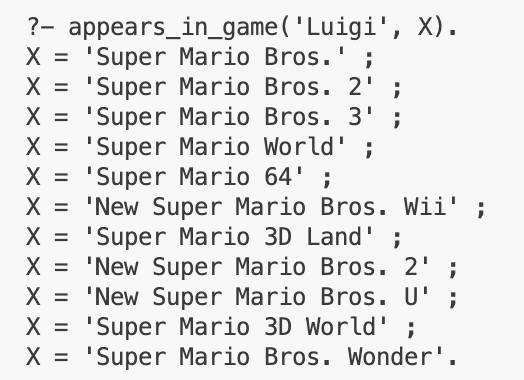
\includegraphics[width=0.5\textwidth]{image/prolog-test-1.png}
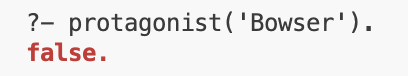
\includegraphics[width=0.5\textwidth]{image/prolog-test-2.png}

\includegraphics[width=\textwidth]{image/prolog-test-3.png}
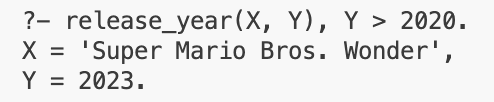
\includegraphics[width=0.5\textwidth]{image/prolog-test-4.png}
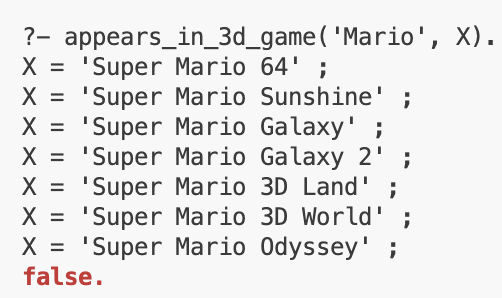
\includegraphics[width=0.5\textwidth]{image/prolog-test-5.png}

\includegraphics[width=\textwidth]{image/prolog-test-6.png}
\nparagraph{Онтология:}
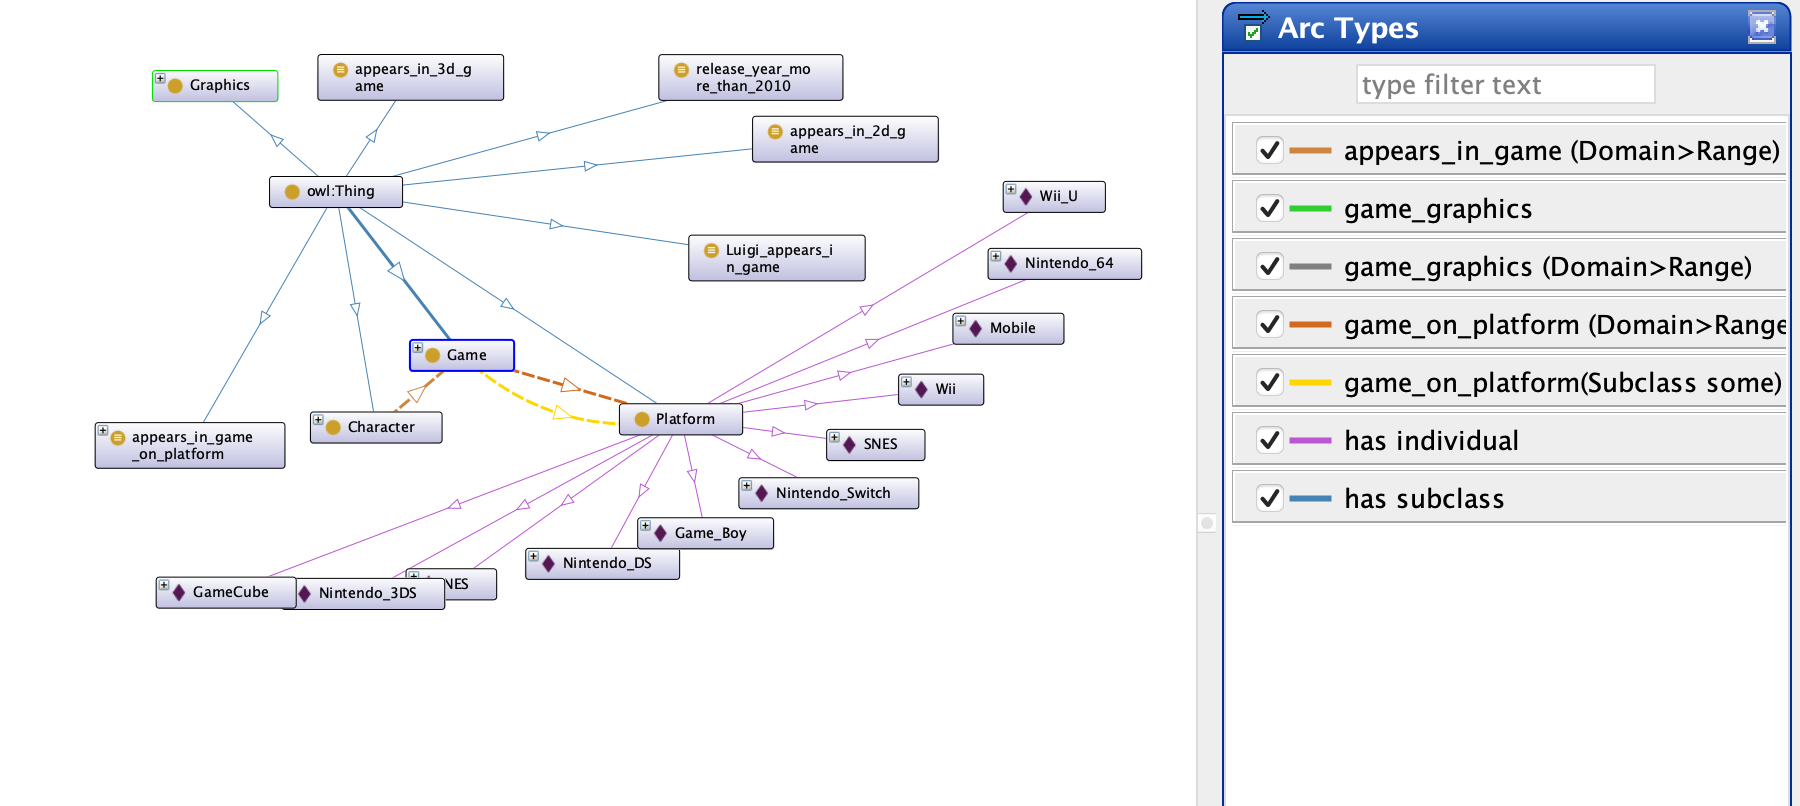
\includegraphics[width=\textwidth]{image/ontology-1.png}
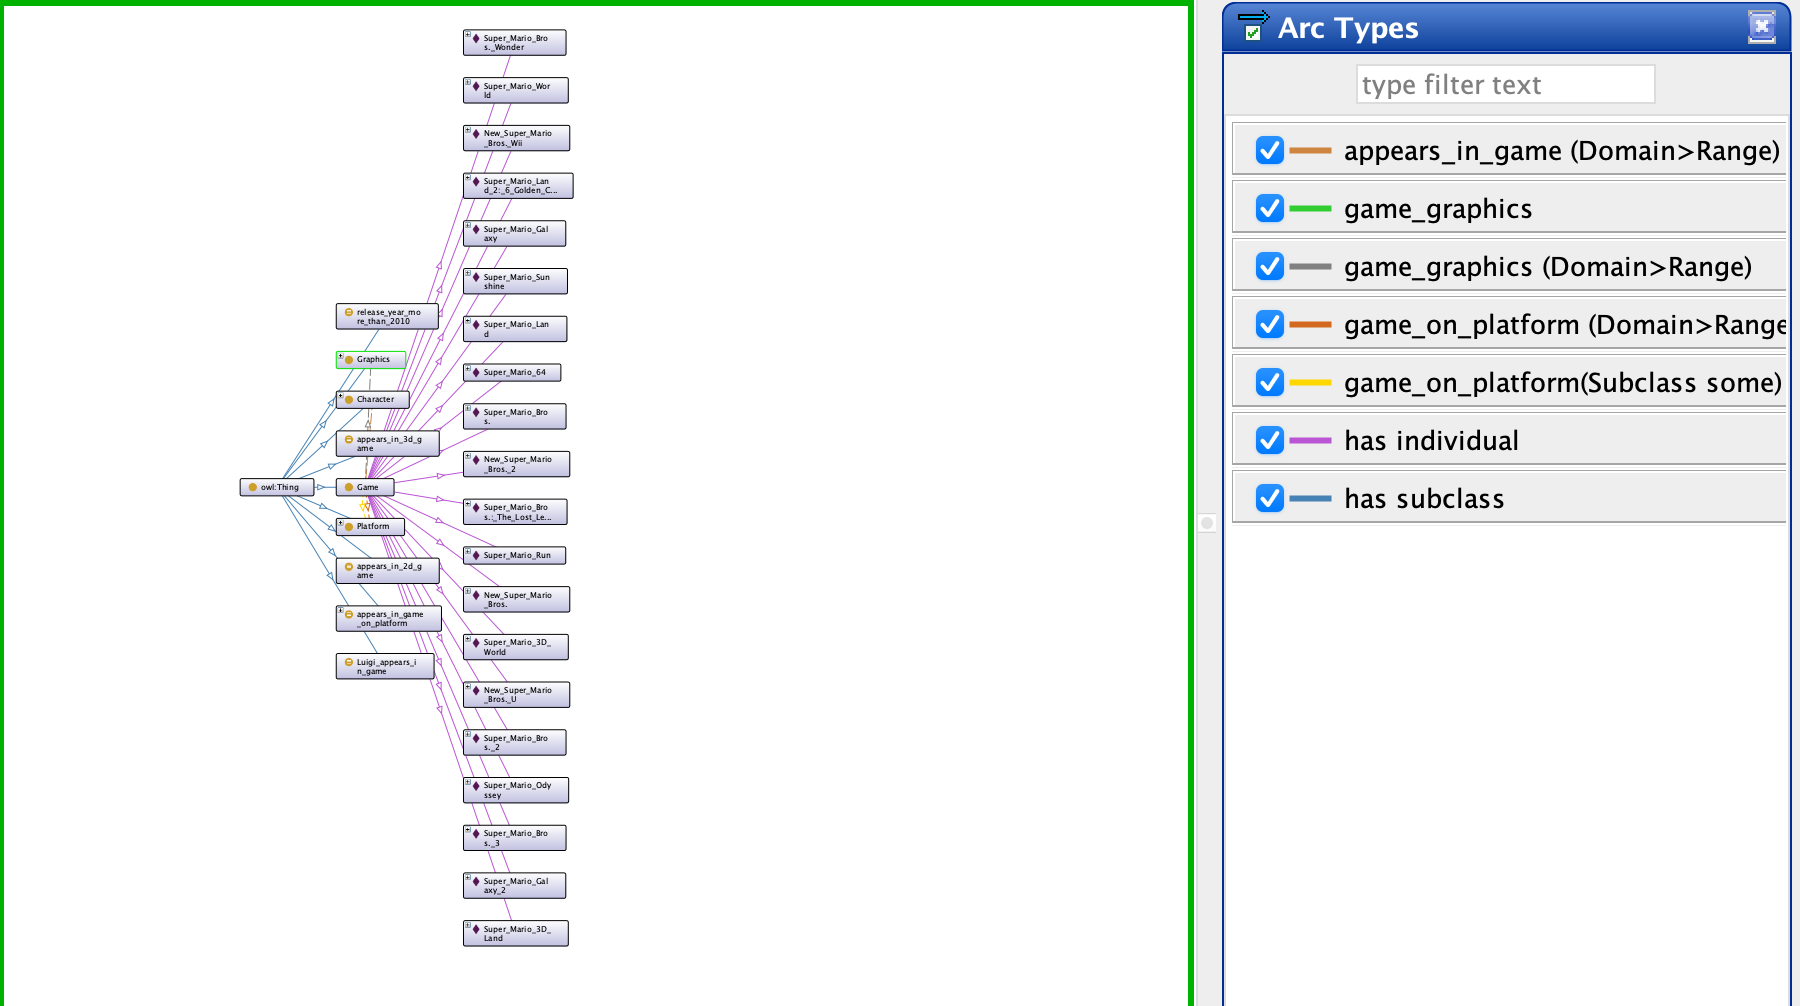
\includegraphics[width=\textwidth]{image/ontology-2.png}
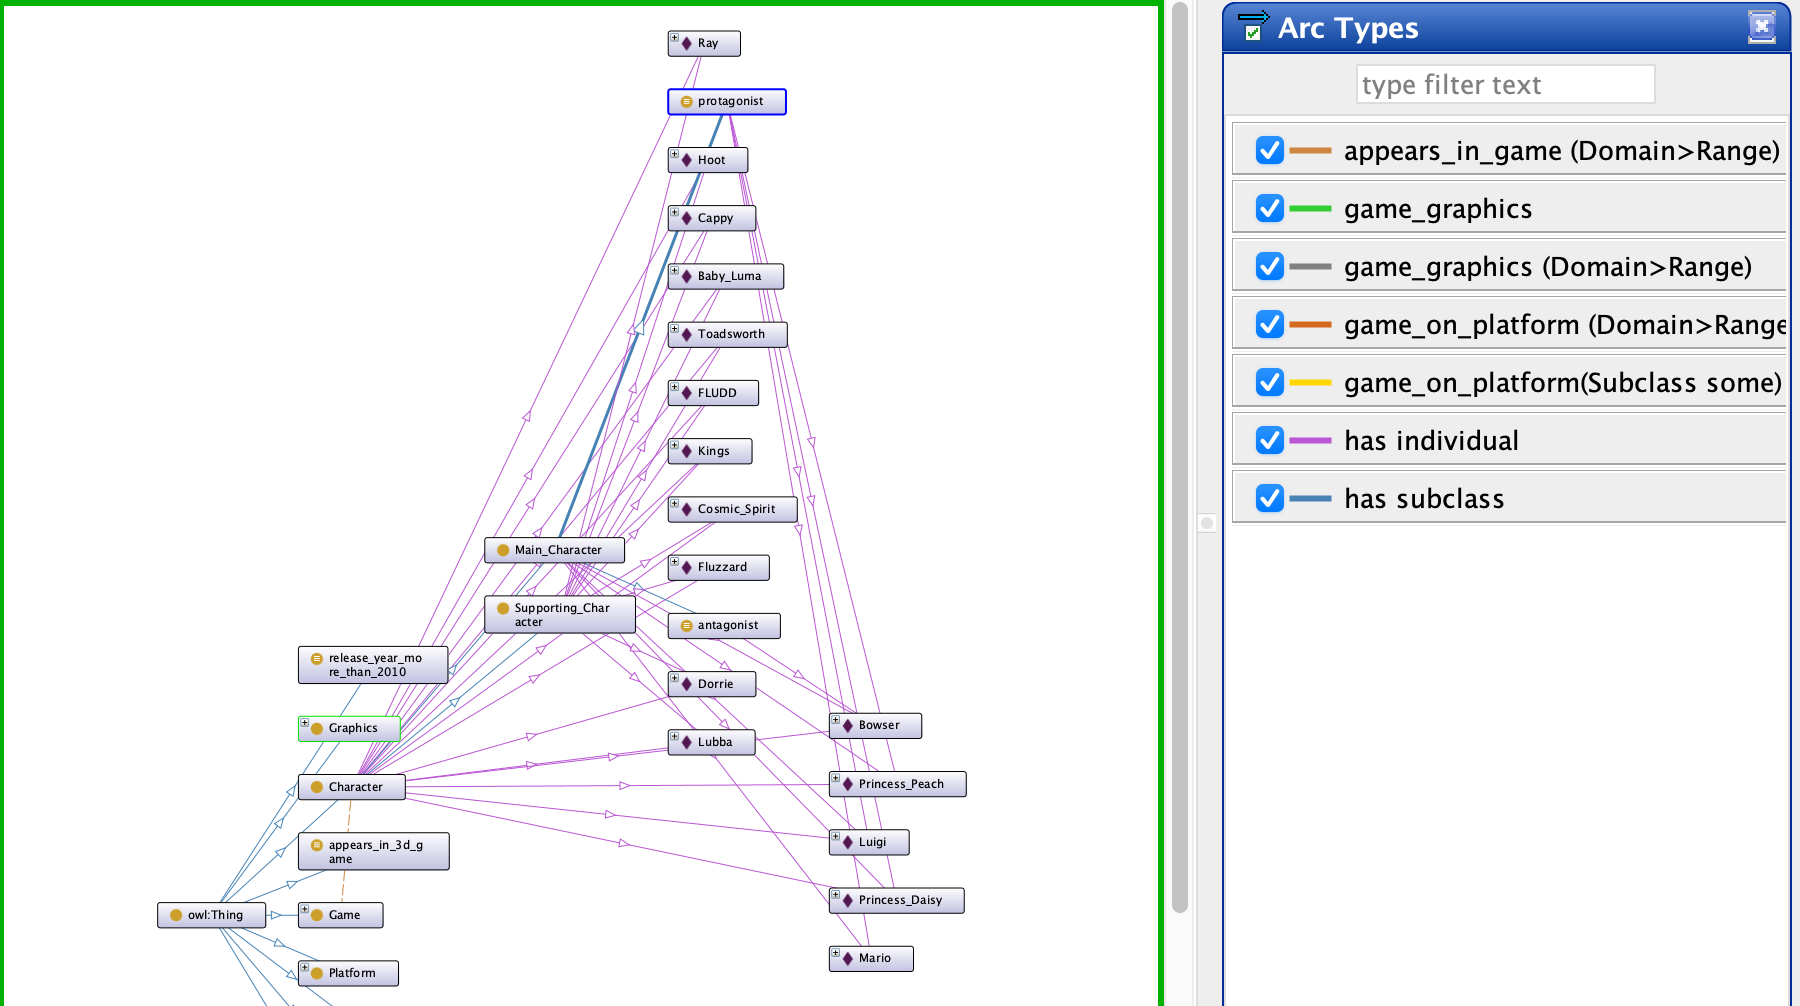
\includegraphics[width=\textwidth]{image/ontology-3.png}
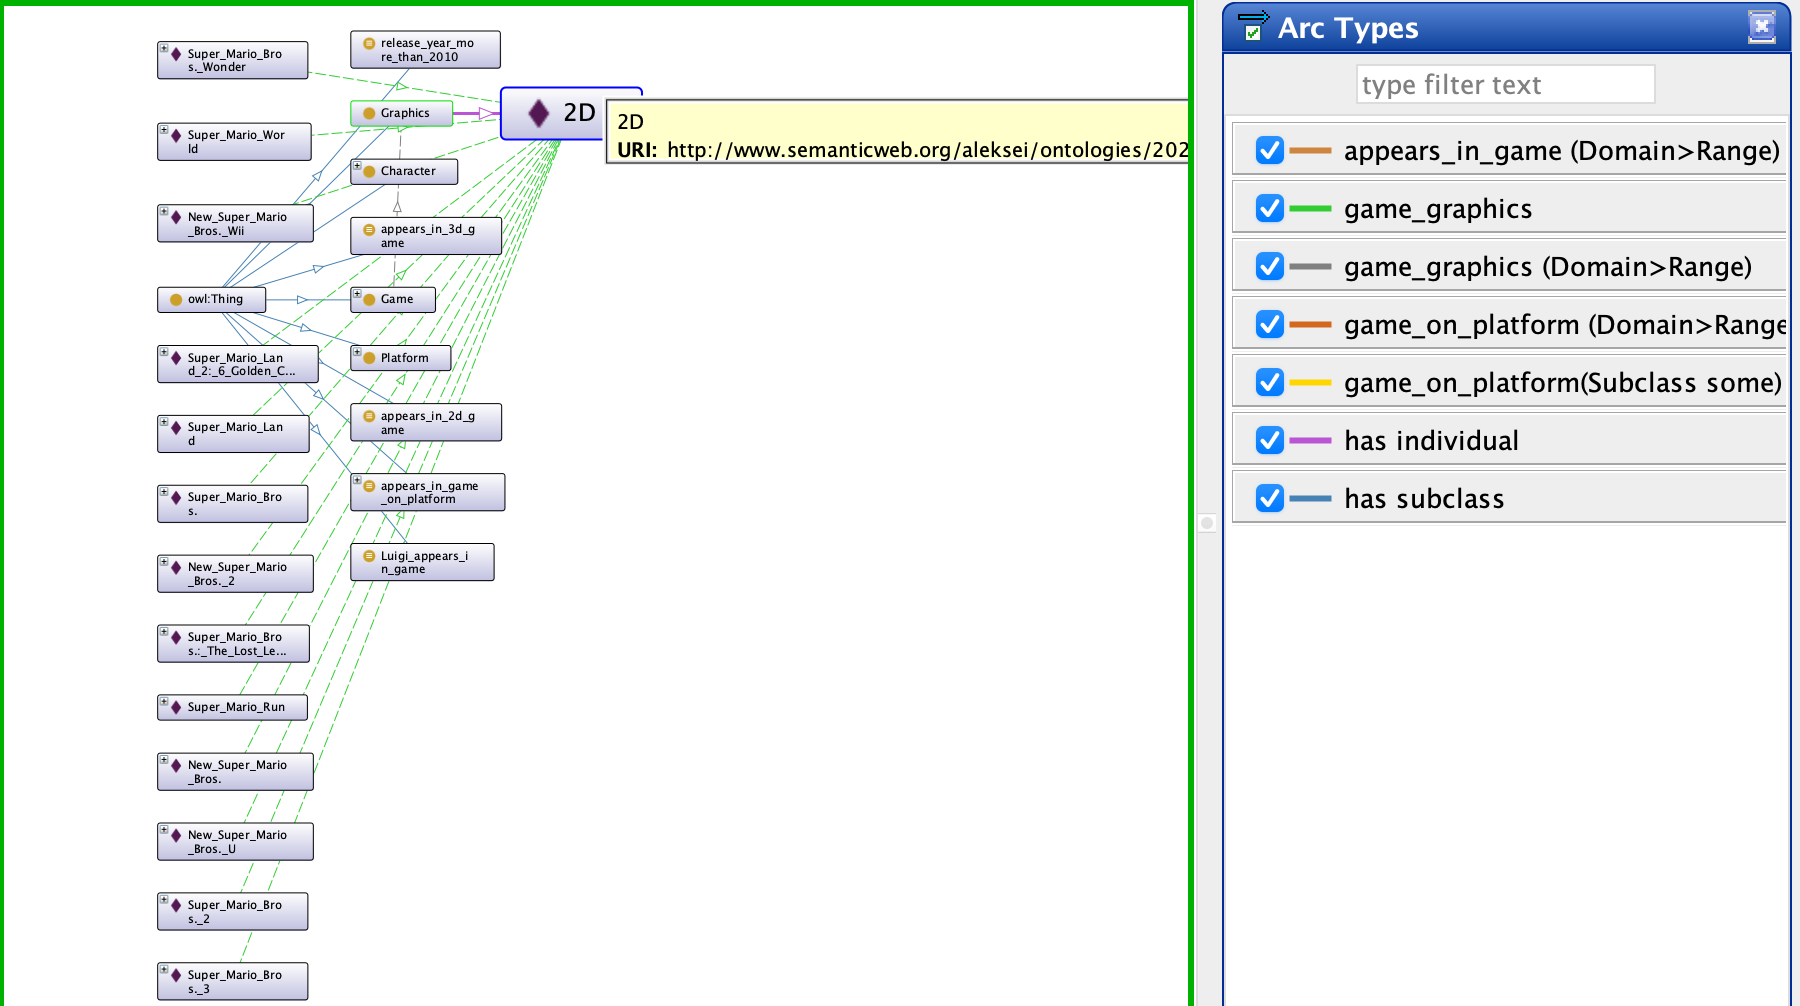
\includegraphics[width=\textwidth]{image/ontology-4.png}
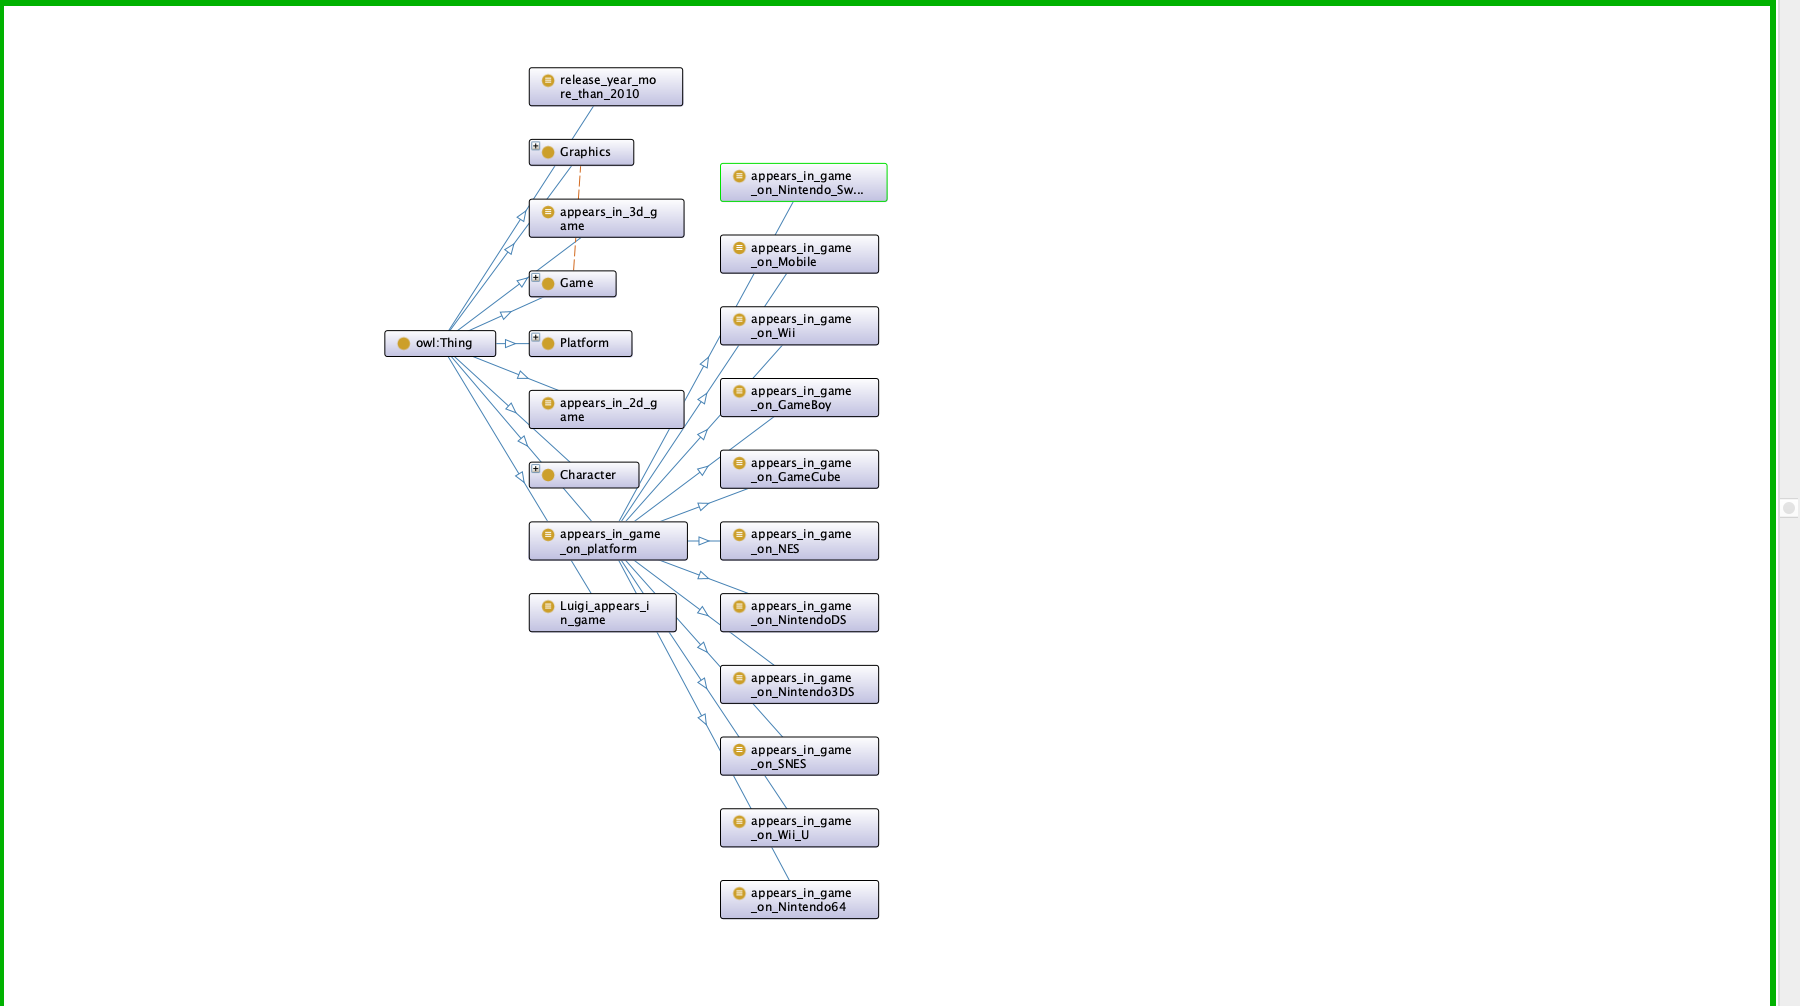
\includegraphics[width=\textwidth]{image/ontology-5.png}
\subparagraph{Тестирование и отладка системы, обеспечение ее функциональности и эффективности.}\mbox{}\\
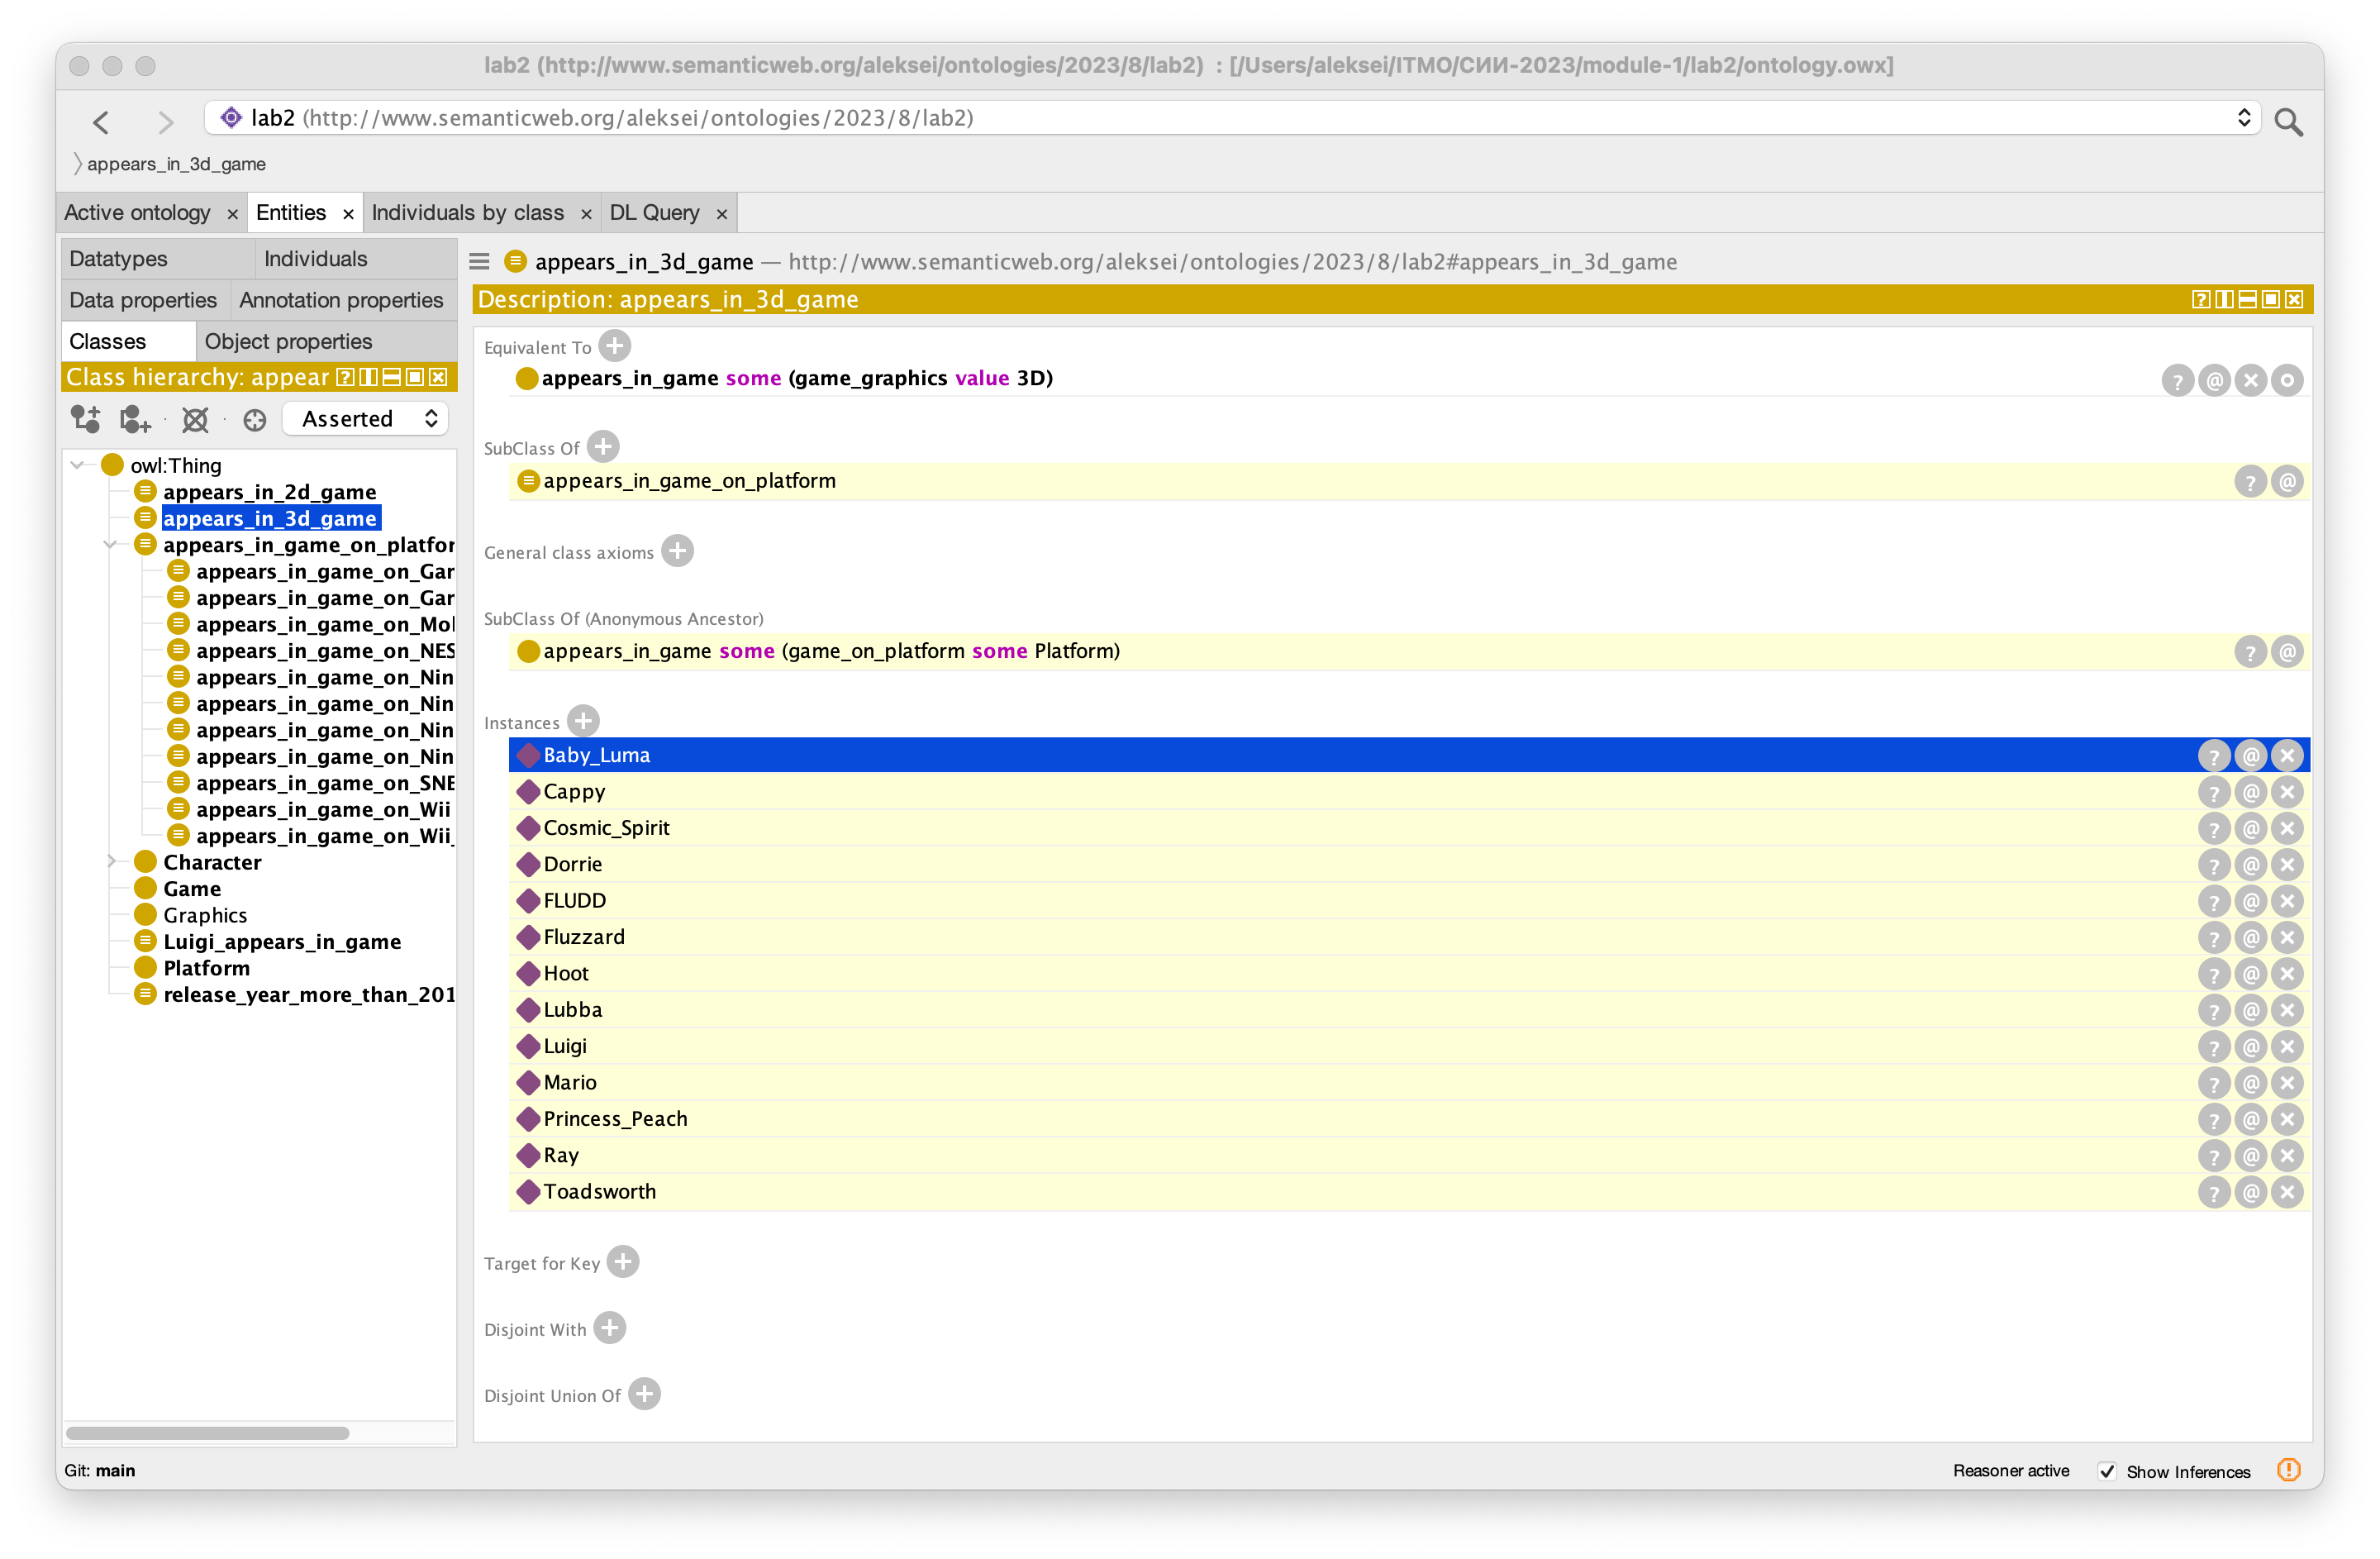
\includegraphics[width=\textwidth]{image/ontology-test-1.png}
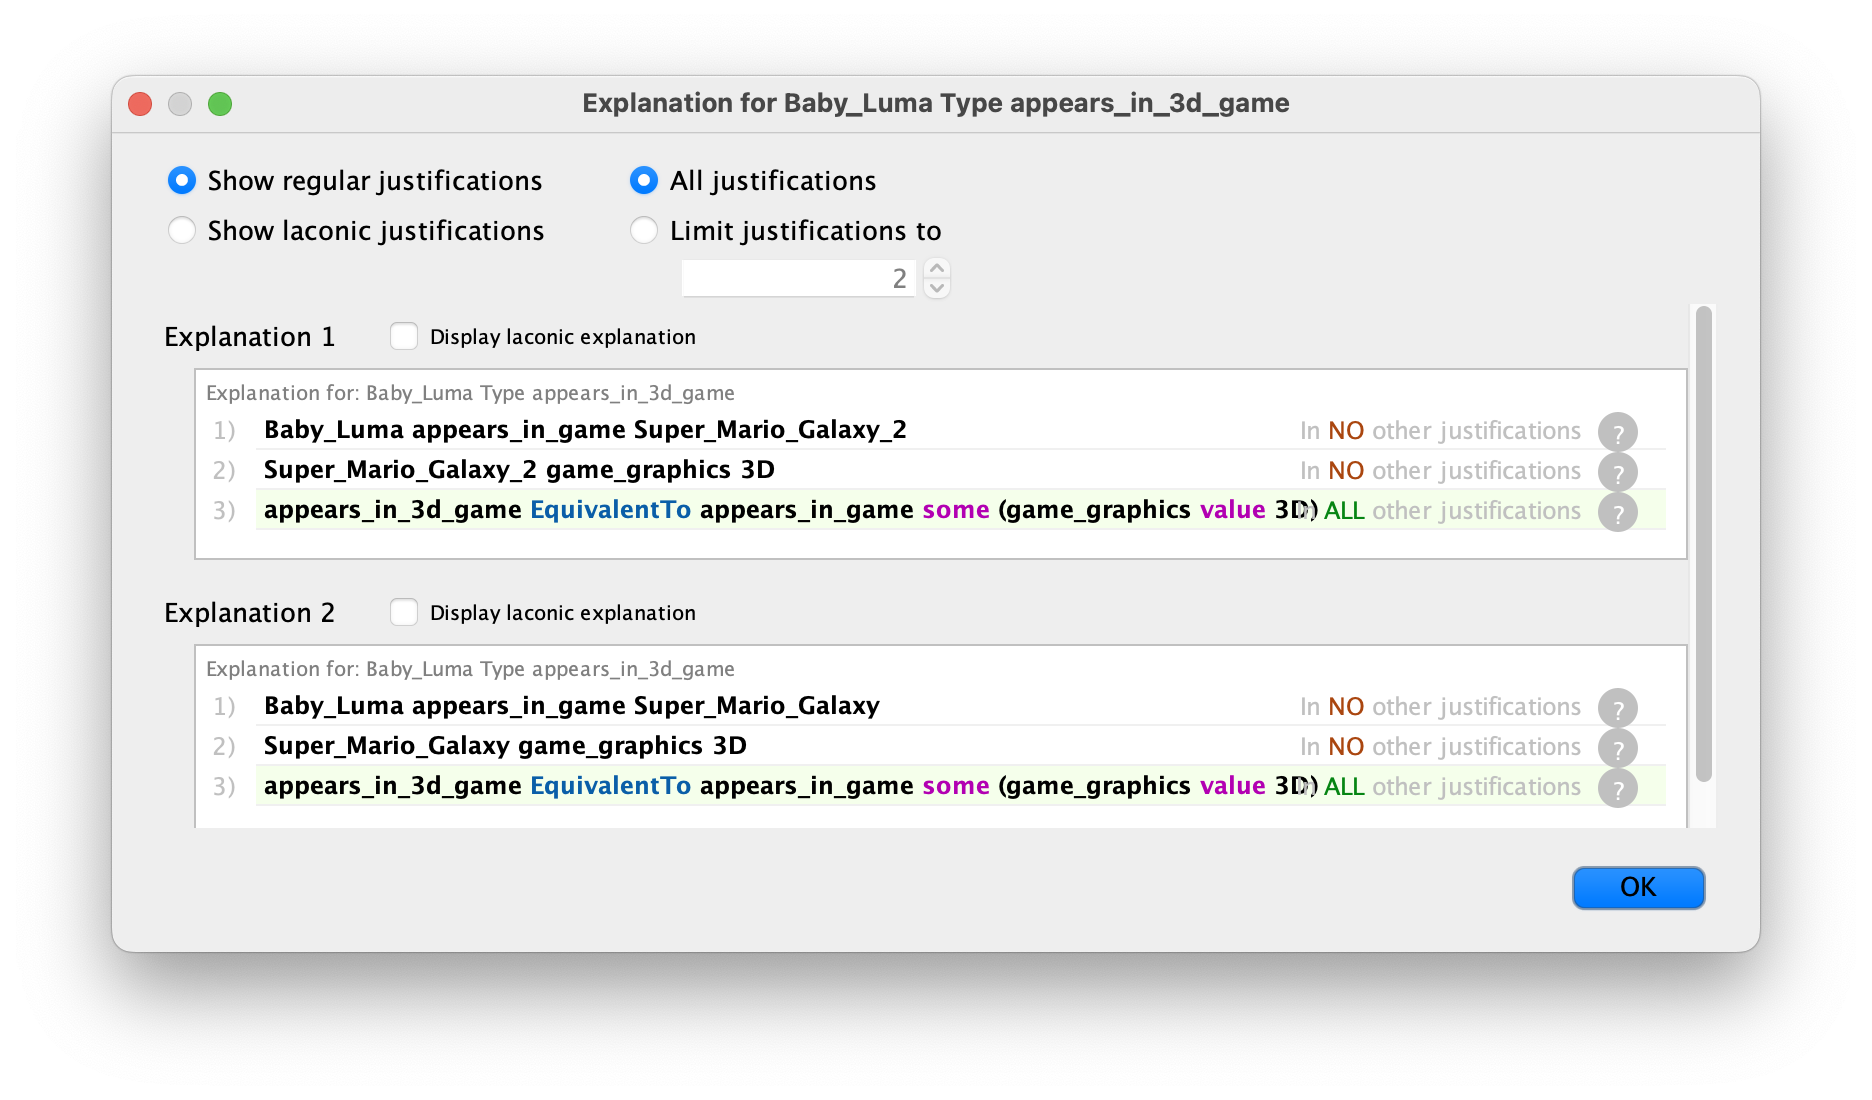
\includegraphics[width=\textwidth]{image/ontology-test-2.png}
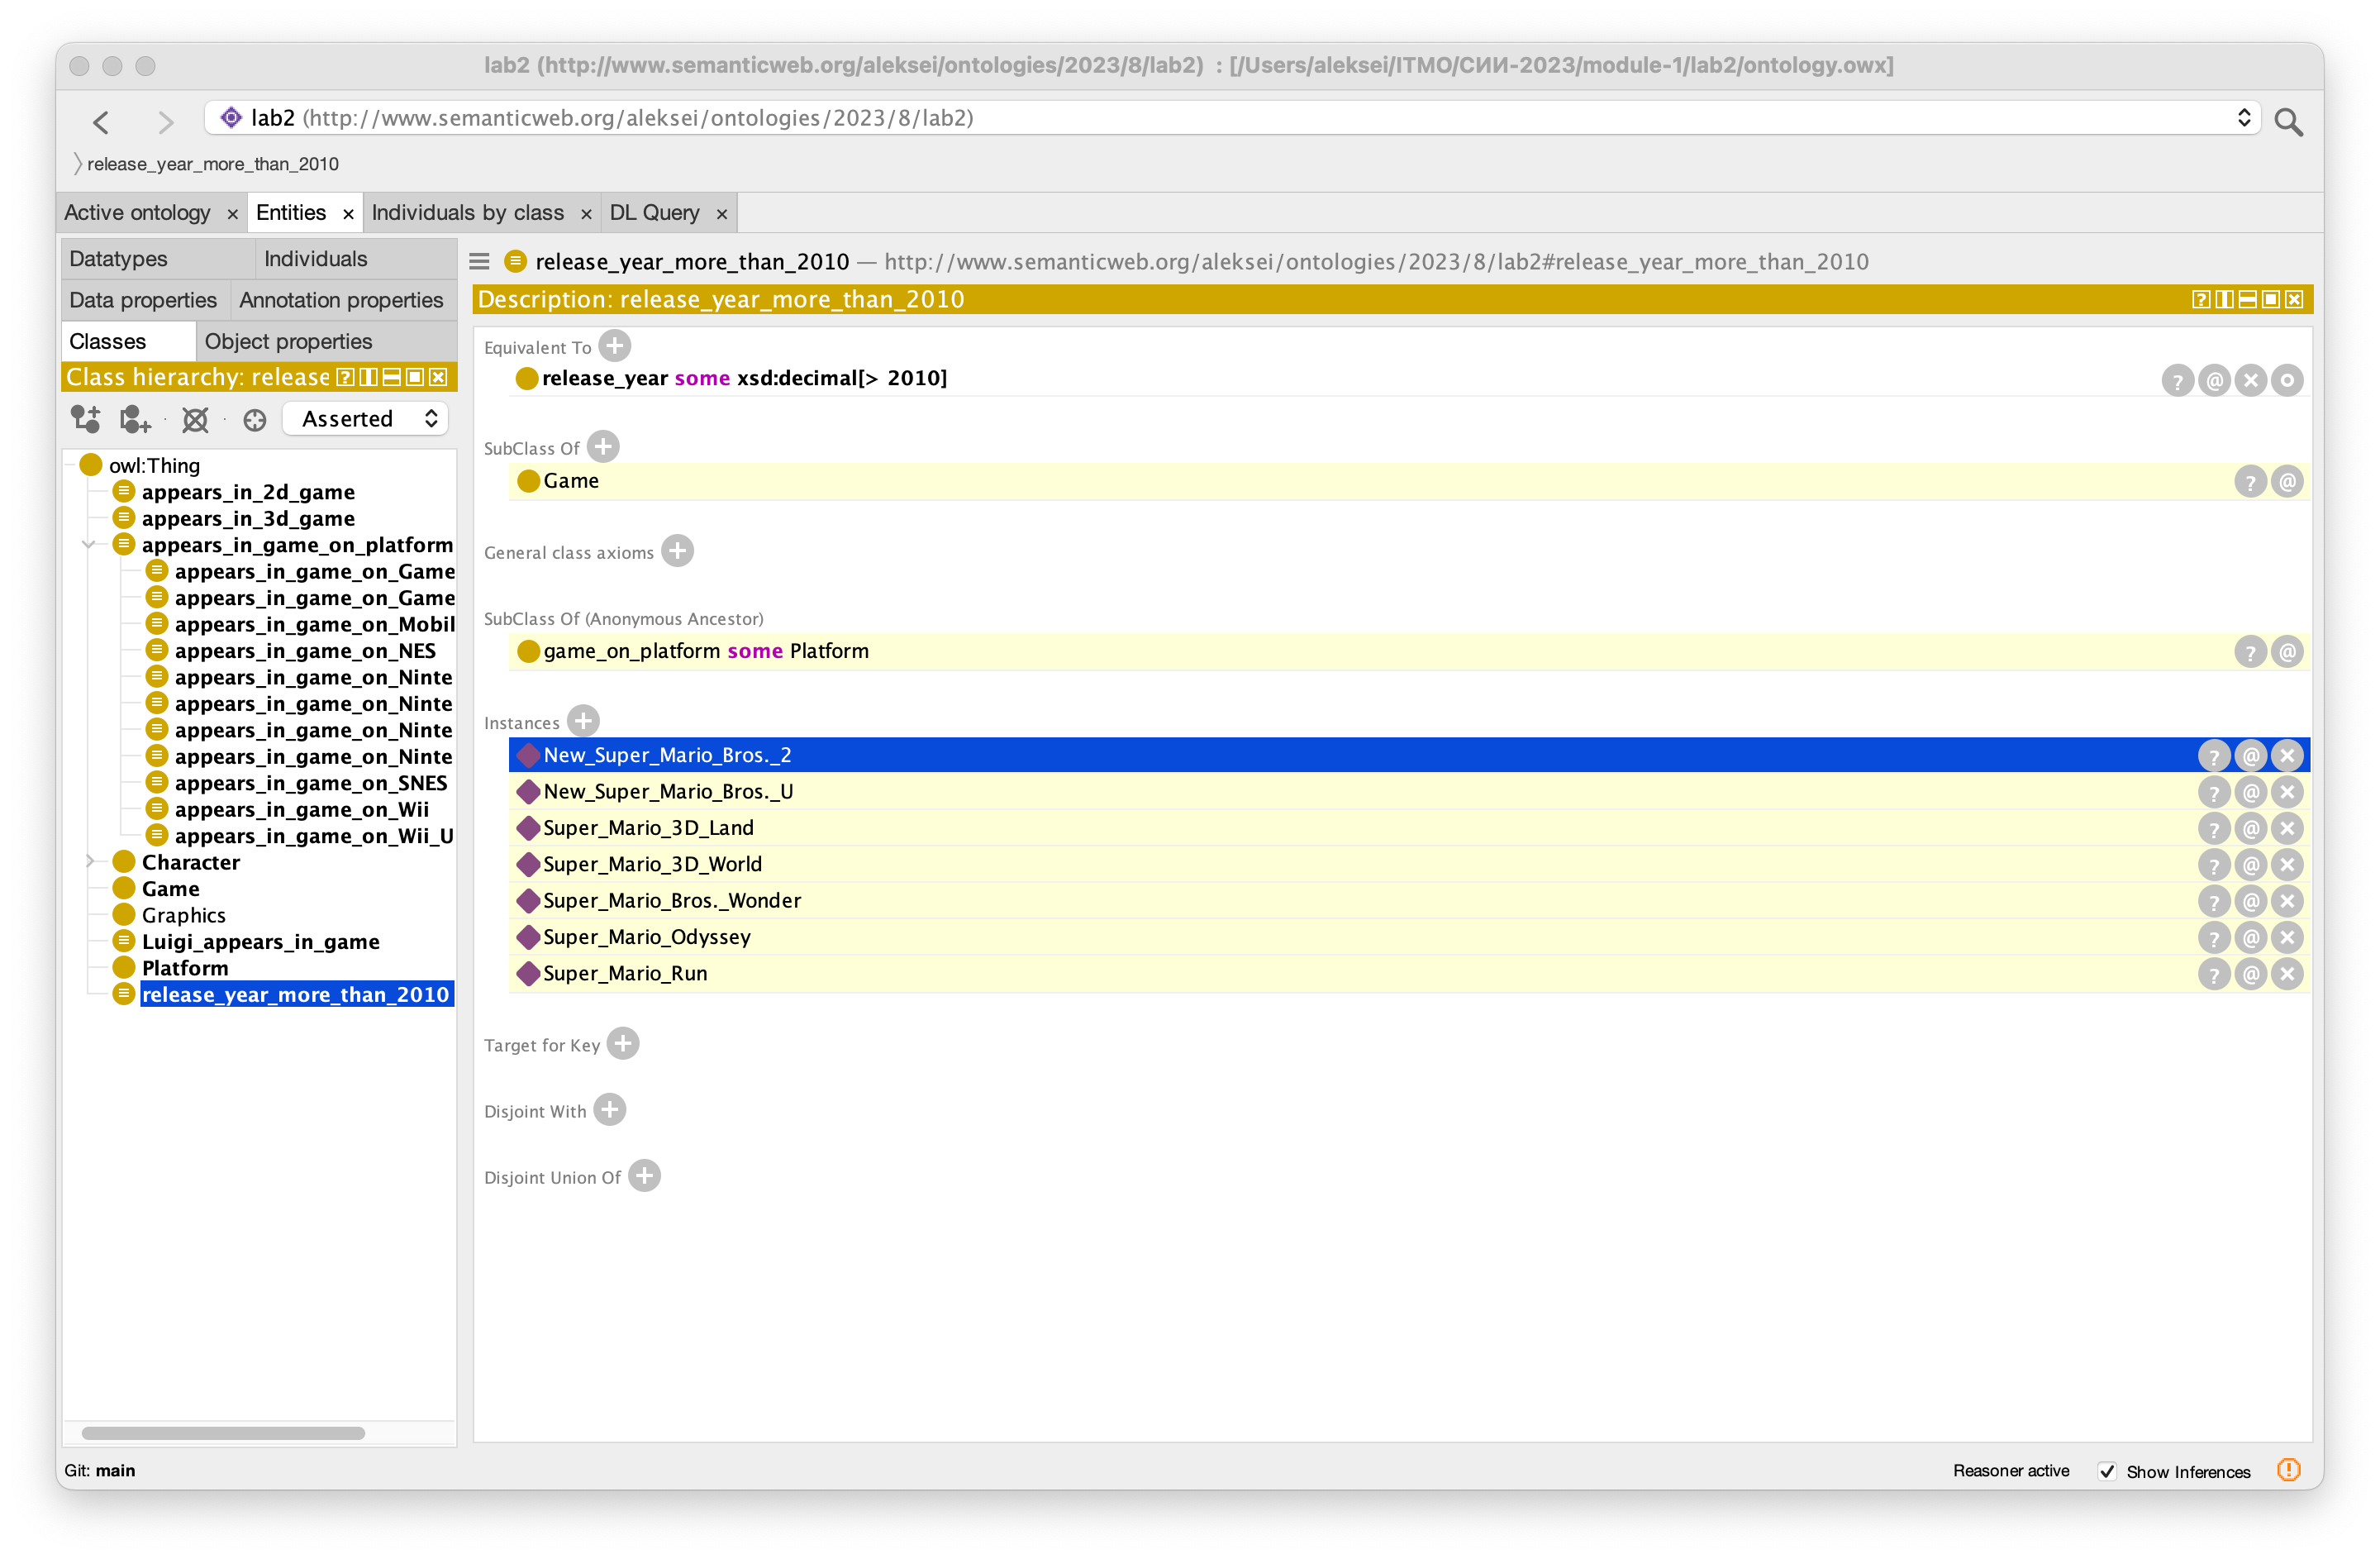
\includegraphics[width=\textwidth]{image/ontology-test-3.png}
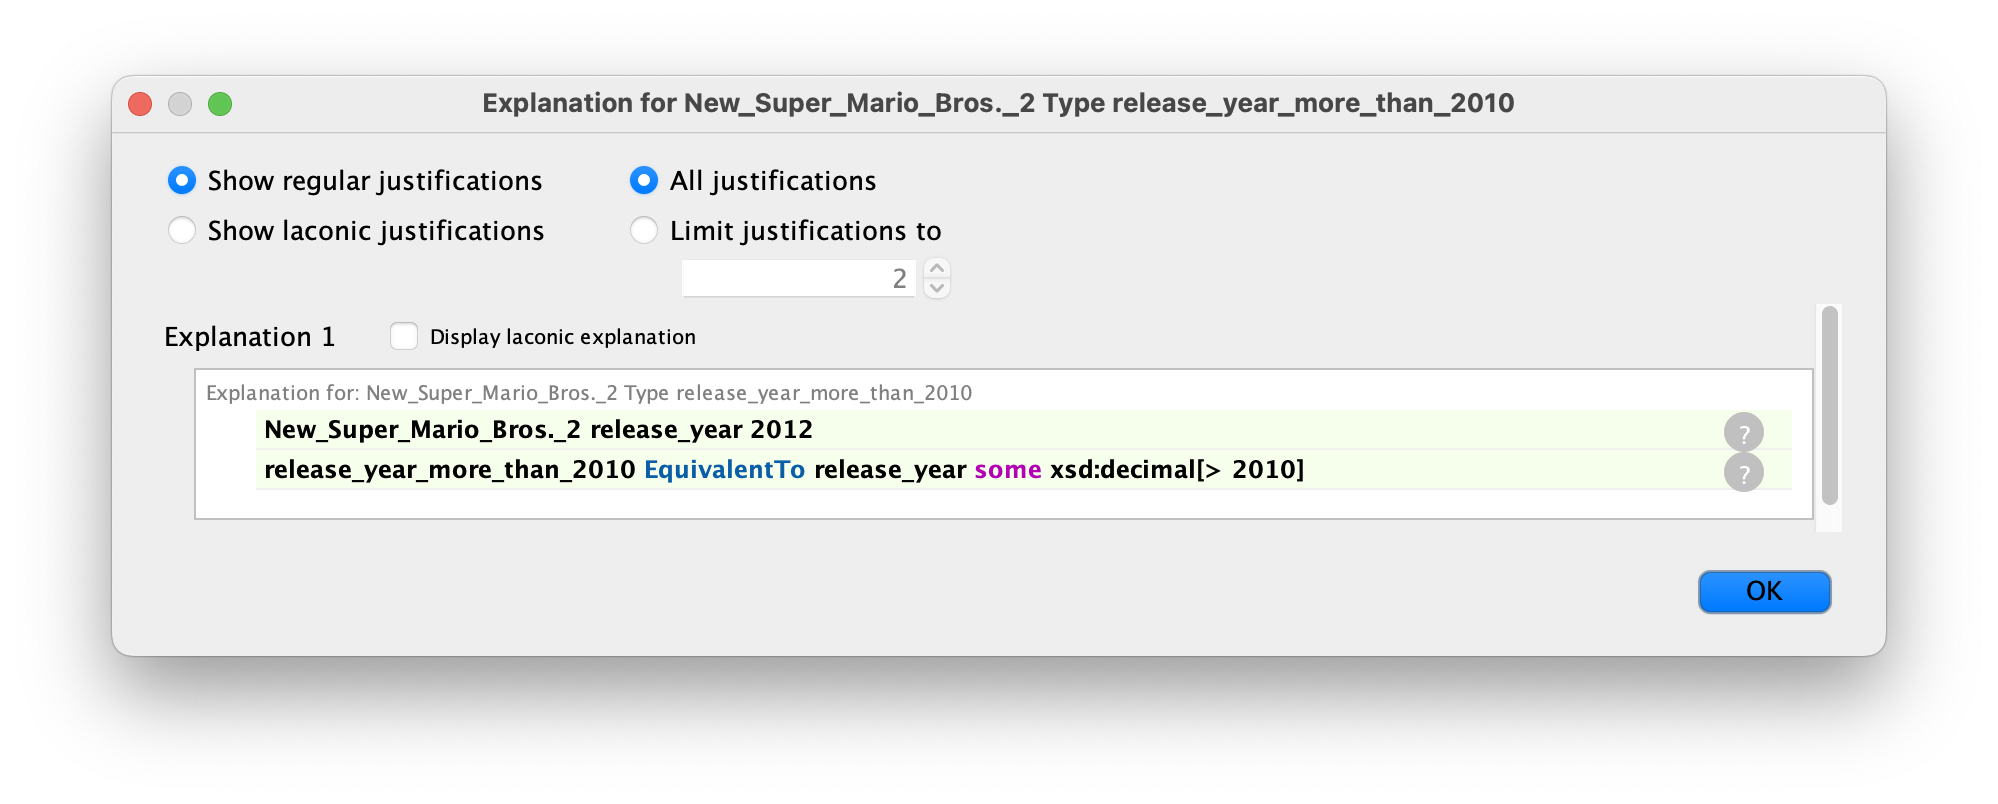
\includegraphics[width=\textwidth]{image/ontology-test-4.png}
\nparagraph{Система поддержки принятия решения на основе базы знаний:}
\lstdefinestyle{java}{language=Java, 
  basicstyle=\small\ttfamily,
  commentstyle=\color{cyan},
  stringstyle=\color{magenta}\ttfamily,
  keywordstyle=\color{blue},
  numbers=left,
  numberstyle=\scriptsize,
  numbersep=5pt,
  frame=single,
  breaklines=true,
  breakatwhitespace=true,
  showstringspaces=false,
  tabsize=4,
  inputencoding=utf8,
  extendedchars=true,
  literate={а}{{\selectfont\char224}}1
          {б}{{\selectfont\char225}}1
          {в}{{\selectfont\char226}}1
          {г}{{\selectfont\char227}}1
          {д}{{\selectfont\char228}}1
          {е}{{\selectfont\char229}}1
          {ё}{{\"e}}1
          {ж}{{\selectfont\char230}}1
          {з}{{\selectfont\char231}}1
          {и}{{\selectfont\char232}}1
          {й}{{\selectfont\char233}}1
          {к}{{\selectfont\char234}}1
          {л}{{\selectfont\char235}}1
          {м}{{\selectfont\char236}}1
          {н}{{\selectfont\char237}}1
          {о}{{\selectfont\char238}}1
          {п}{{\selectfont\char239}}1
          {р}{{\selectfont\char240}}1
          {с}{{\selectfont\char241}}1
          {т}{{\selectfont\char242}}1
          {у}{{\selectfont\char243}}1
          {ф}{{\selectfont\char244}}1
          {х}{{\selectfont\char245}}1
          {ц}{{\selectfont\char246}}1
          {ч}{{\selectfont\char247}}1
          {ш}{{\selectfont\char248}}1
          {щ}{{\selectfont\char249}}1
          {ъ}{{\selectfont\char250}}1
          {ы}{{\selectfont\char251}}1
          {ь}{{\selectfont\char252}}1
          {э}{{\selectfont\char253}}1
          {ю}{{\selectfont\char254}}1
          {я}{{\selectfont\char255}}1
          {А}{{\selectfont\char192}}1
          {Б}{{\selectfont\char193}}1
          {В}{{\selectfont\char194}}1
          {Г}{{\selectfont\char195}}1
          {Д}{{\selectfont\char196}}1
          {Е}{{\selectfont\char197}}1
          {Ё}{{\"E}}1
          {Ж}{{\selectfont\char198}}1
          {З}{{\selectfont\char199}}1
          {И}{{\selectfont\char200}}1
          {Й}{{\selectfont\char201}}1
          {К}{{\selectfont\char202}}1
          {Л}{{\selectfont\char203}}1
          {М}{{\selectfont\char204}}1
          {Н}{{\selectfont\char205}}1
          {О}{{\selectfont\char206}}1
          {П}{{\selectfont\char207}}1
          {Р}{{\selectfont\char208}}1
          {С}{{\selectfont\char209}}1
          {Т}{{\selectfont\char210}}1
          {У}{{\selectfont\char211}}1
          {Ф}{{\selectfont\char212}}1
          {Х}{{\selectfont\char213}}1
          {Ц}{{\selectfont\char214}}1
          {Ч}{{\selectfont\char215}}1
          {Ш}{{\selectfont\char216}}1
          {Щ}{{\selectfont\char217}}1
          {Ъ}{{\selectfont\char218}}1
          {Ы}{{\selectfont\char219}}1
          {Ь}{{\selectfont\char220}}1
          {Э}{{\selectfont\char221}}1
          {Ю}{{\selectfont\char222}}1
          {Я}{{\selectfont\char223}}1
}
\lstinputlisting[style=java]{../lab3/src/main/java/org/lapin/Main.java}
\lstinputlisting[style=java]{../lab3/src/main/java/org/lapin/parser/Parser.java}
\subparagraph{Тестирование и отладка системы, обеспечение ее функциональности и эффективности.}
\begin{verbatim}
Hello and welcome!
Enter your query: 
Мой любимый персонаж: Mario, Luigi - у меня есть приставка: NES, Nintendo DS
 - я люблю играть в игры с графикой: 2D, 3D.
Вам подойдут игры: 
'Super Mario Bros.'
'Super Mario Bros.: The Lost Levels'
'Super Mario Bros. 2'
'Super Mario Bros. 3'
'New Super Mario Bros.'
'Super Mario Bros.'
'Super Mario Bros. 2'
'Super Mario Bros. 3'
\end{verbatim}
\begin{verbatim}
Hello and welcome!
Enter your query: 
Я люблю играть в игры с графикой: 3D - Мой любимый персонаж: Mario, Luigi 
и Princess Peach
Вам подойдут игры: 
'Super Mario 64'
'Super Mario 64'
'Super Mario Sunshine'
'Super Mario Galaxy'
'Super Mario Galaxy 2'
'Super Mario 3D Land'
'Super Mario 3D Land'
'Super Mario 3D World'
'Super Mario 3D World'
'Super Mario Odyssey'
\end{verbatim}
\section{Оценка и интерпретация результатов:}
\subsection{Примеры запросов для БЗ и онтологии, сравнение разницы реализации.}
\nparagraph{Запрос к базе знаний:}
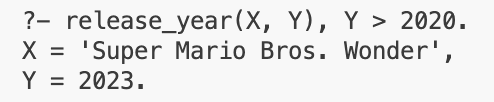
\includegraphics[width=\textwidth]{image/prolog-test-4.png}
\nparagraph{Запрос к онтологии:}
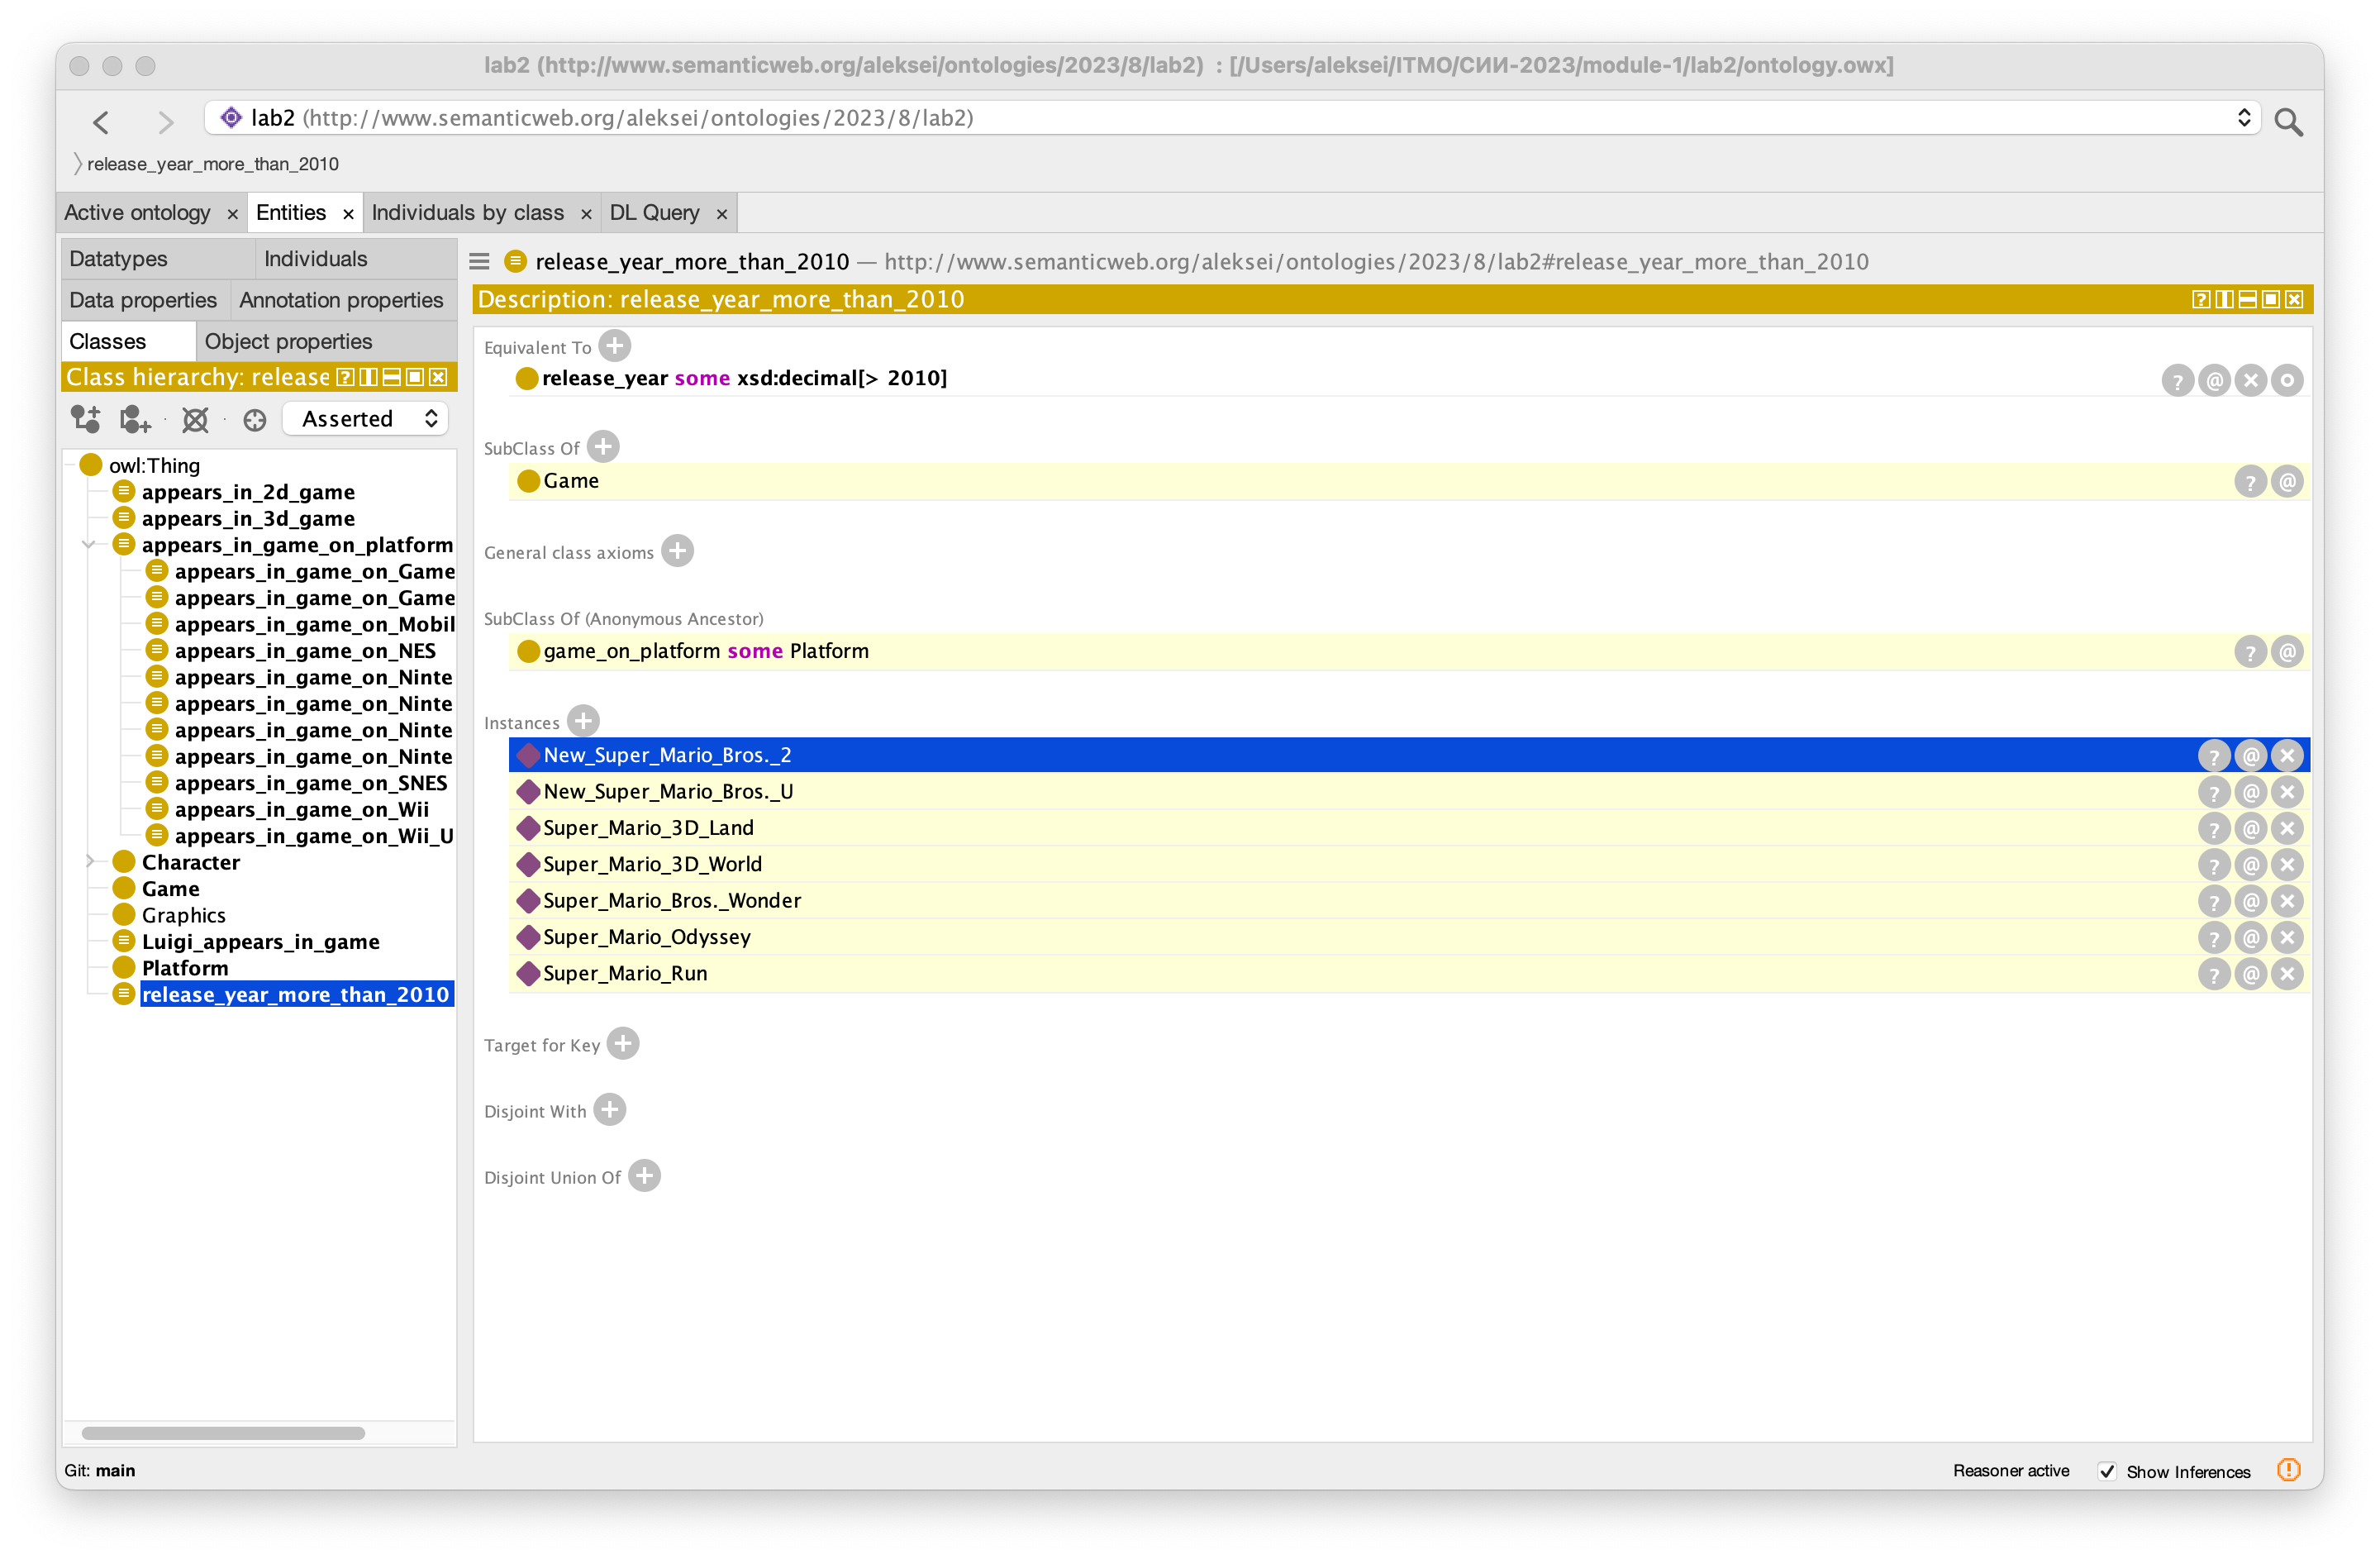
\includegraphics[width=\textwidth]{image/ontology-test-3.png}
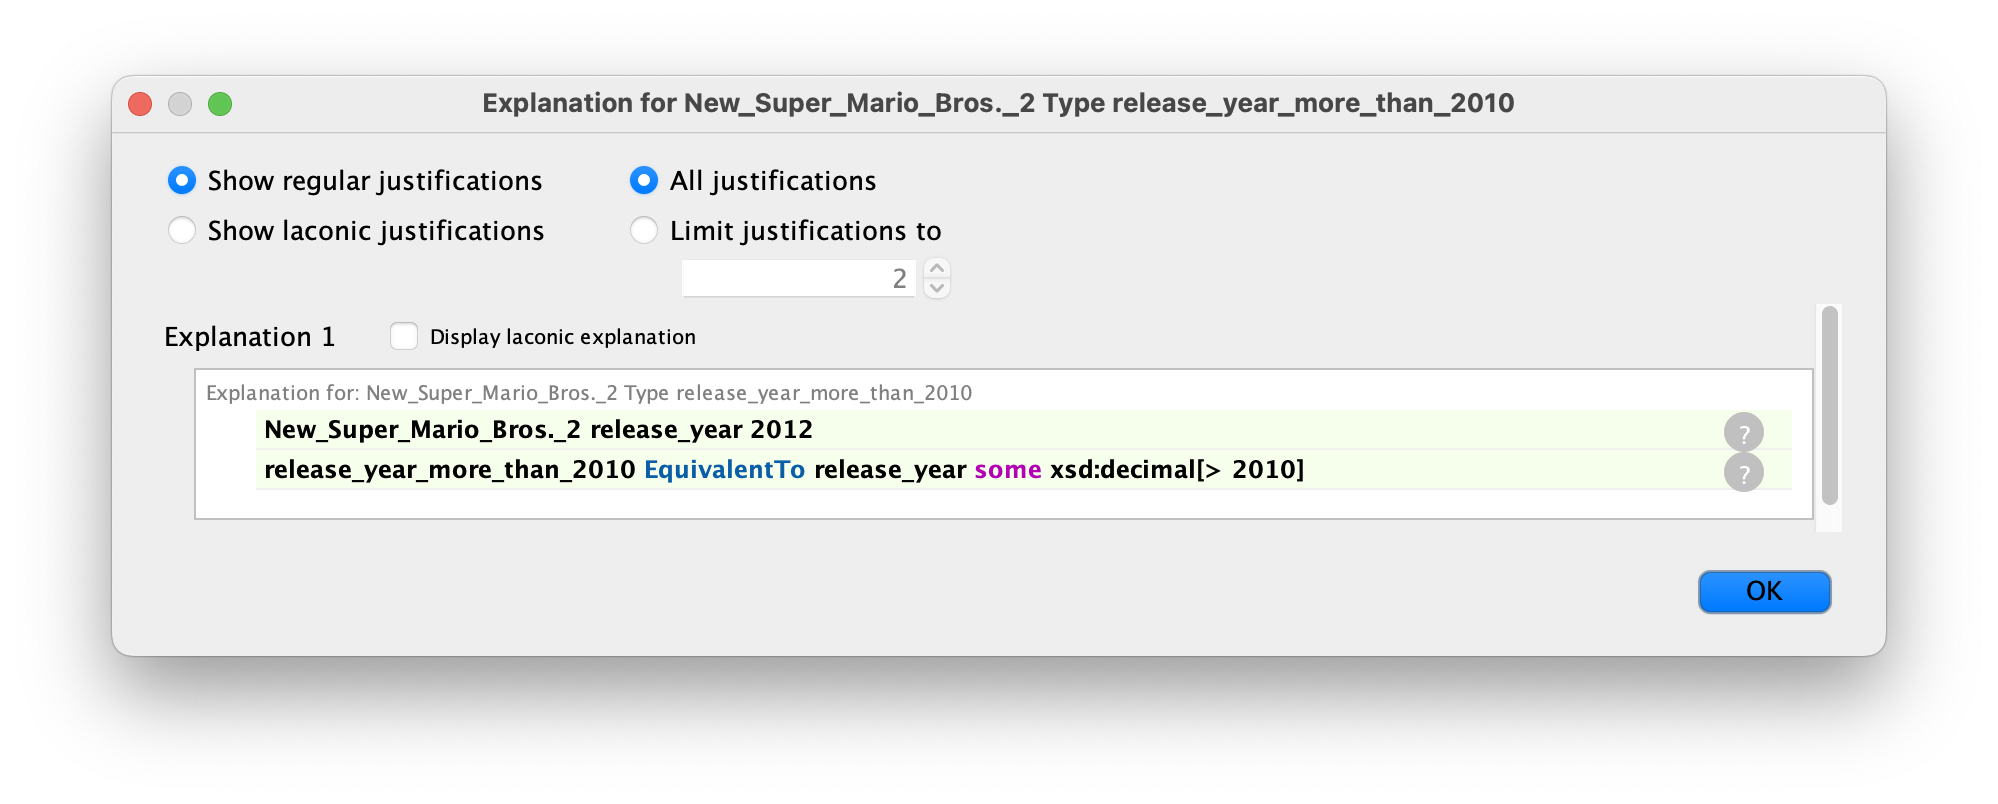
\includegraphics[width=\textwidth]{image/ontology-test-4.png}
Реализация запроса через факт в Prolog и свойства в Protege похожи.
\nparagraph{Запрос к базе знаний:}
\begin{verbatim}
% Rule: Character appears in a Super Mario game released on a specific platform
appears_in_game_on_platform(X, Y) :- appears_in_game(X, Z), game_on_platform(Z, Y).
\end{verbatim}

\includegraphics[width=\textwidth]{image/prolog-test-3.png}
\nparagraph{Запрос к онтологии:}
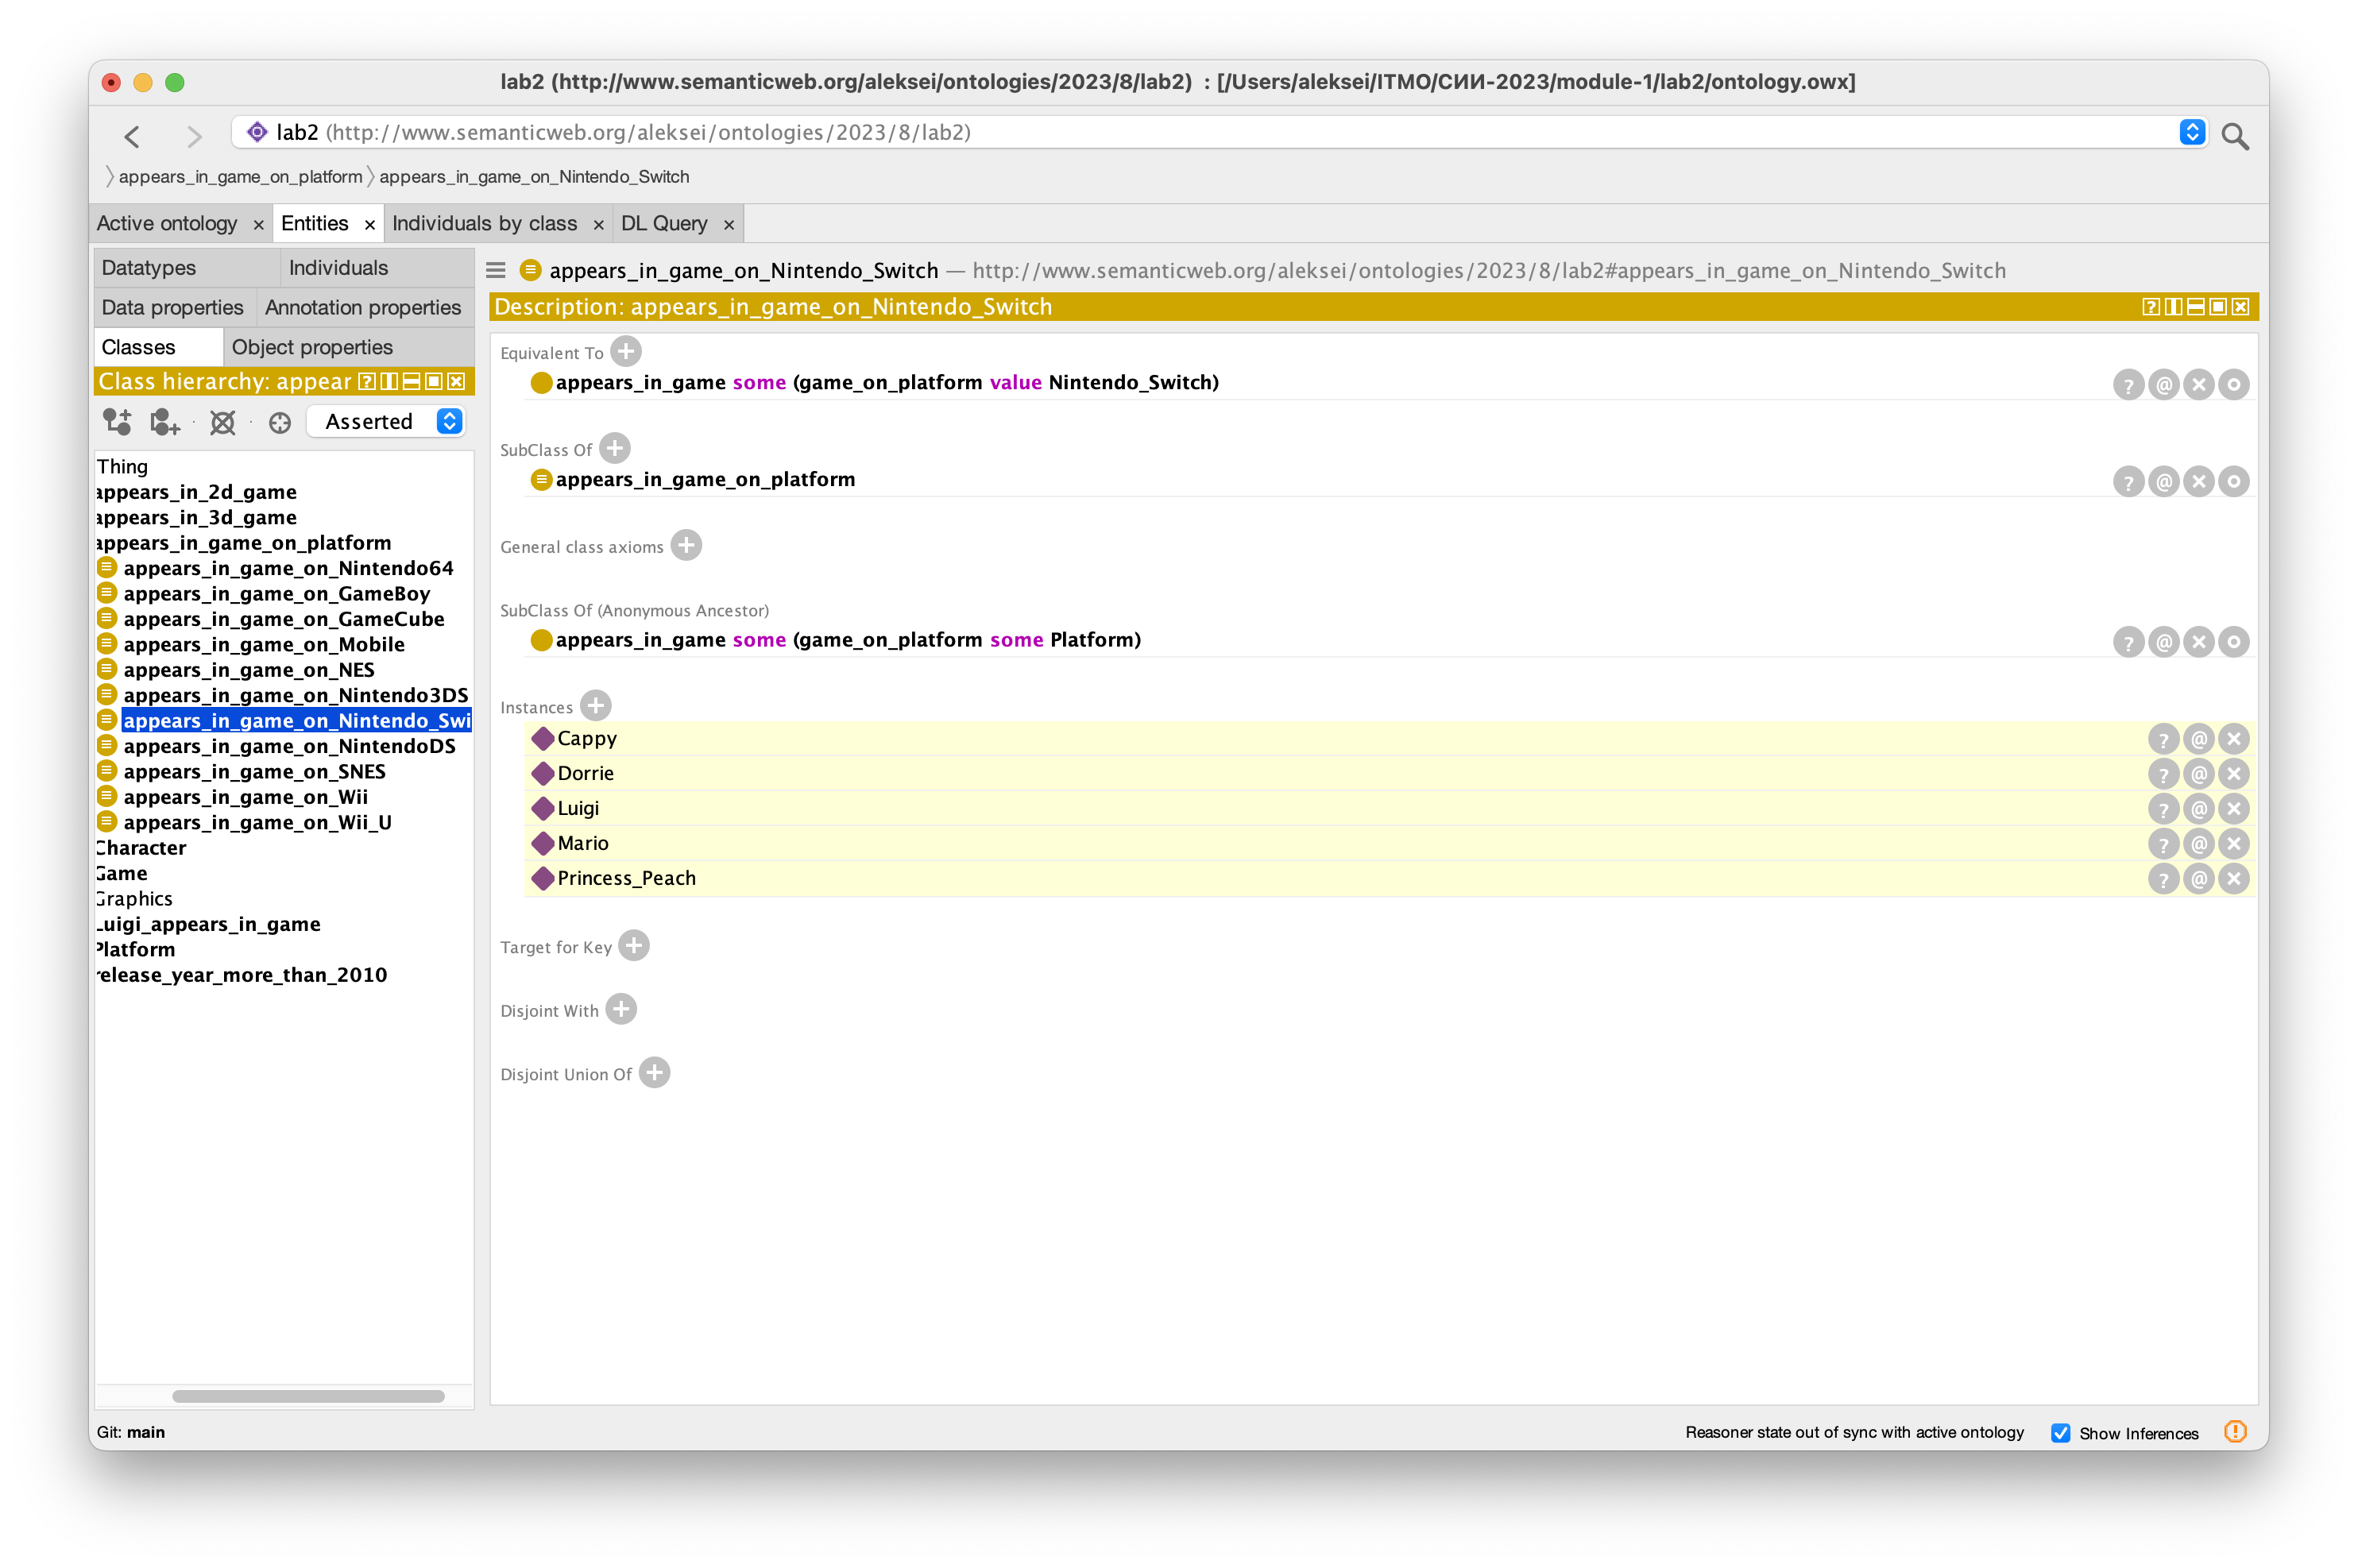
\includegraphics[width=\textwidth]{image/ontology-test-5.png}
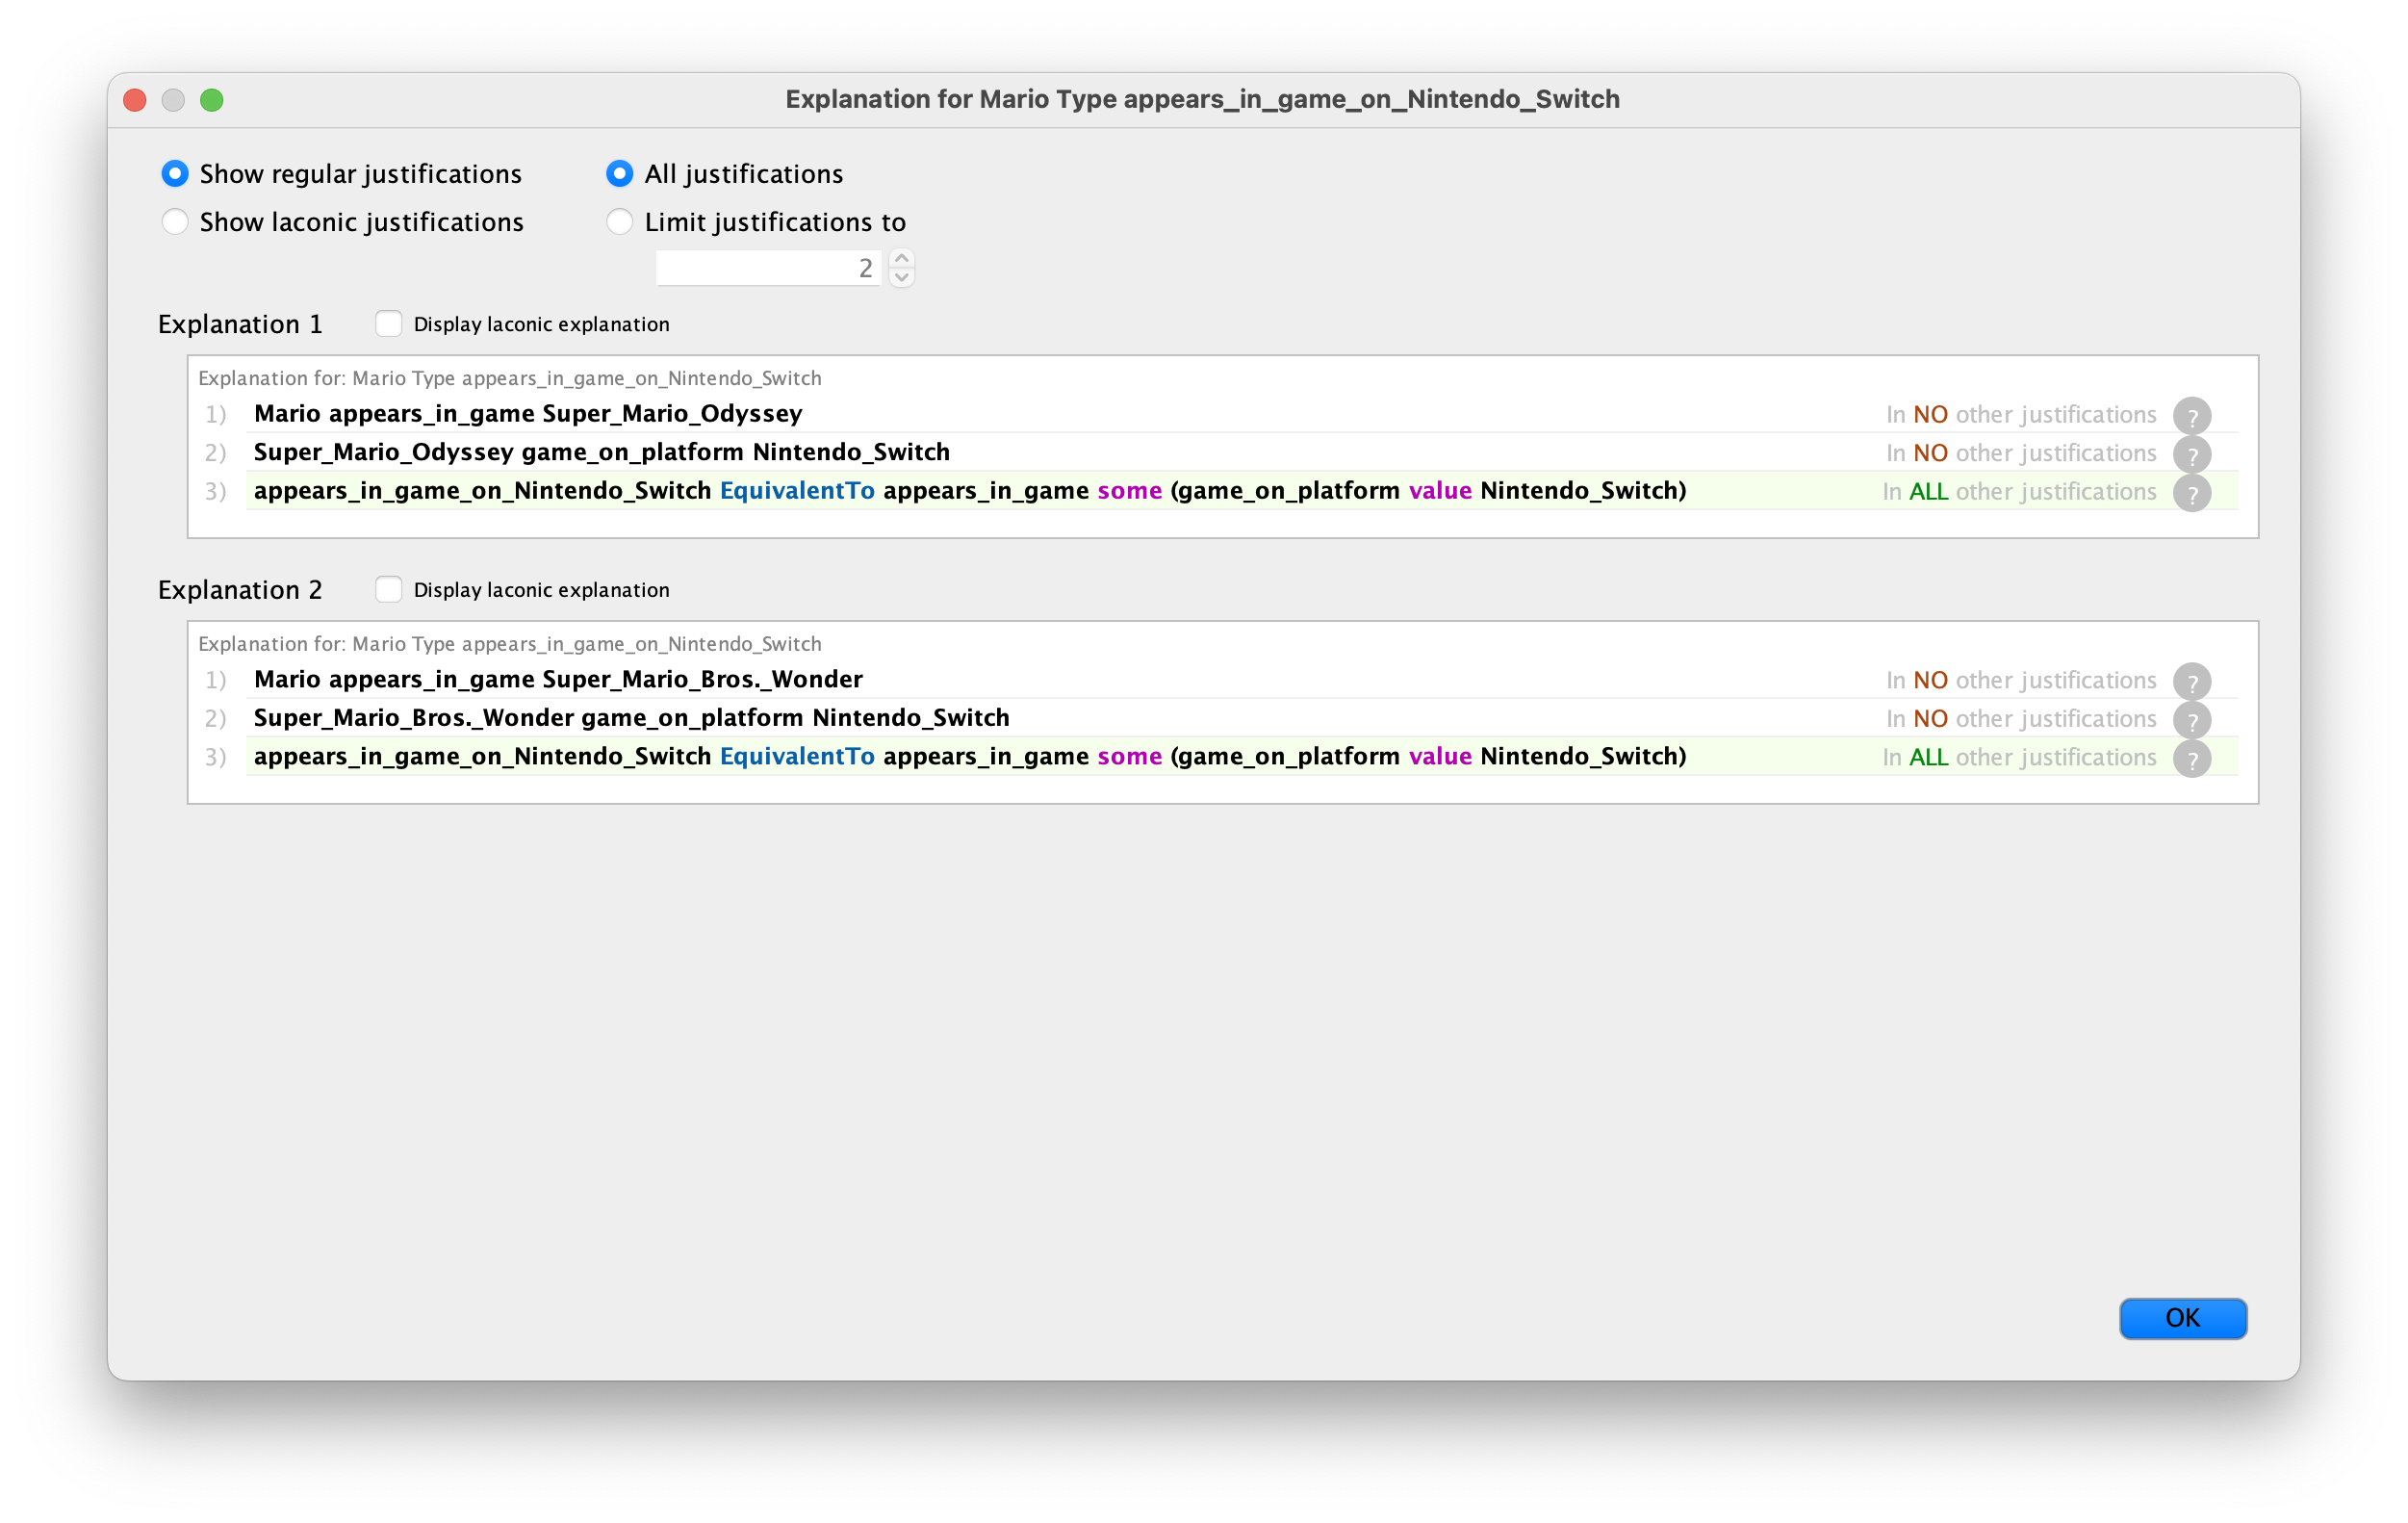
\includegraphics[width=\textwidth]{image/ontology-test-6.png}
Реализация запроса через правило в Prolog, отличается в удобстве использования от реализация через отдельные классы эквивалентные определенным правилам для каждой платформы.
\subsection{Оценка соответствия системы поставленным требованиям и достижению целей проекта.}
Система способна обрабатывать запросы пользователей, связанные с играми серии Super Mario, и выдавать релевантные рекомендации. Была реализована база знаний на языке Prolog и онтология на языке OWL с помощью Protege, которые позволяют хранить и структурировать информацию о персонажах, играх и платформах серии Super Mario.\\
Также была реализована система поддержки принятия решения на основе базы знаний, которая позволяют находить игры, соответствующие запросам пользователей. Были проведены тесты системы, которые показали ее эффективность и корректность.\\
Таким образом, система полностью соответствует поставленным требованиям и целям проекта, и может быть использована для обработки запросов пользователей, связанных с играми серии Super Mario.\\
Система поддержки принятия решений на основе базы знаний соответствует основным требованиям, таким как:
\begin{itemize}
  \item Принимает запросы пользователя через командную строку и обрабатывает их с помощью парсера.
  \item Формулирует логические запросы к базе знаний Prolog, используя введенные пользователем данные.
  \item Предоставляет рекомендации, советы, связанные с выбором видеоигры, на основе результатов выполнения запросов.
  \item Есть документация работы системы и описание ее функциональности.
\end{itemize}
Система достигает целей проекта, таких как:
\begin{itemize}
  \item Развитие навыков логического программирования и создания базы знаний на Prolog
  \item Развитие навыков работы с онтологиями и семантическими технологиями
  \item Развитие навыков разработки систем поддержки принятия решений, использующих базу знаний или онтологию для предоставления рекомендаций
  \item Практическое применение системы в помощи пользователям при выборе видеоигр
\end{itemize}
\subsection{Интерпретация результатов и описание дальнейших возможностей развития и улучшения системы.}

В результате разработки системы поддержки принятия решений на основе базы знаний и онтологии для выбора видеоигр серии Super Mario были достигнуты поставленные цели и требования проекта. Система успешно обрабатывает запросы пользователей и предоставляет рекомендации, соответствующие их запросам.\\

Однако, существуют возможности для дальнейшего улучшения и развития системы. Например, можно добавить больше информации о персонажах, играх и платформах серии Super Mario, чтобы система могла предоставлять более точные и полезные рекомендации. Также можно улучшить парсер запросов, чтобы система могла обрабатывать более сложные запросы и предоставлять более точные результаты.\\

Кроме того, можно рассмотреть возможность интеграции системы с другими сервисами и платформами, такими как онлайн-магазины игр, чтобы пользователи могли сразу же приобрести рекомендованные игры. Также можно рассмотреть возможность добавления функционала для сравнения игр и выбора наиболее подходящей для пользователя.\\

В целом, система поддержки принятия решений на основе базы знаний и онтологии для выбора видеоигр серии Super Mario является успешным проектом, который может быть дальше улучшен и развит для удовлетворения потребностей пользователей.\\

\section{Заключение:}
\subsection{Описание преимуществ и потенциальных применений разработанной системы искусственного интеллекта на базе Prolog, баз знаний и онтологий.}
\nparagraph{Преимущества системы:}
\begin{itemize}
  \item Система позволяет пользователю получать рекомендации по выбору видеоигр на основе своих интересов и предпочтений, используя логический язык Prolog и базу знаний, содержащую информацию о различных играх серии Super Mario.
  \item Система использует декларативный подход к представлению знаний, что упрощает их описание и обновление. Система также способна проводить логический вывод и унификацию для поиска решения.
  \item Система демонстрирует возможности Prolog и семантических технологий для разработки систем искусственного интеллекта, таких как экспертные системы, рекомендательные системы, системы обработки естественного языка и другие
  \item Система имеет практическое значение для пользователей, которые хотят найти подходящую видеоигру из серии Super Mario
\end{itemize}
\nparagraph{Потенциальные применения системы:}
\begin{itemize}
  \item Система может быть использована для помощи пользователям в выборе видеоигр не только из серии Super Mario, но и из других жанров и франшиз, расширяя базу знаний или онтологию соответствующими данными.
  \item Система может быть интегрирована с другими приложениями и сервисами, такими как веб-сайты, мобильные приложения, голосовые ассистенты и социальные сети.
\end{itemize}
\end{document}
